% DECISION: MLSys'27 research track (author, 2026-10-15): the MLSys 2025 style files, which the MLSys 2027 call names; two columns, at most 10 pages before the references; double-blind.
%% Template: mlsys2025.sty and mlsys2025.bst copied unchanged from media.mlsys.org/Conferences/MLSYS2025/mlsys2025style.zip (sha256 04e77090...ba3768ef); algorithm, algorithmic, and fancyhdr come from TeX Live.
\documentclass{article}

\usepackage{microtype}
\usepackage{graphicx}
\usepackage{booktabs}
\usepackage{array}
\usepackage{amsmath}
\usepackage{amssymb}
\usepackage{textcomp}
\usepackage{xcolor}
\usepackage{threeparttable}
\usepackage[hyphens]{url}
\usepackage[hidelinks]{hyperref}

%% The template's recommended pairing of hyperref and algorithmic.
\newcommand{\theHalgorithm}{\arabic{algorithm}}

%% The review version; the camera-ready version passes [accepted].
\usepackage{mlsys2025}

% Placeholders: \E marks a value or passage still owed; \figph stands in for a figure not yet drawn.
\newcommand{\E}[1]{\textcolor{red}{$\langle$#1$\rangle$}}
\newcommand{\figph}[2][0.9\linewidth]{\fbox{\parbox[c][3cm][c]{#1}{\centering\small\textcolor{red}{#2}}}}

\newcommand{\us}{\,\textmu{}s}
\newcommand{\ms}{\,ms}

\let\oldtexttt\texttt
\renewcommand{\texttt}[1]{{\small\oldtexttt{#1}}}

\hyphenation{tool-chain}

% VALUE: the acronym is recoverable from the subtitle word for word (OPerator Concurrency from Command ORDer),
% and the subtitle states the paper's thesis: concurrency follows from the order of the commands.
% DECISION: settled by the author with three converging reviews (venue fit, durability in use, accuracy).
% "in Compiled Designs" was cut because "design" is FPGA/AIE vocabulary an ML reader does not parse, because it
% invites the "nothing is recompiled" reading that the split builds contradict, and because it leans
% post-compilation when aie-cosched-schedule is itself a compiler pass. "for Edge LLM Inference" was cut because
% it narrows the line below "AMD AI Engines", which is the architecture family the legality conditions are stated
% over; because truncation eats the trailing scope first and would leave an unscoped claim; and because the draft's
% own word for the setting is "client", with "edge" reserved for the models.
% DECISION: the subtitle carries a verb. Without one it is a statement of subject, and a verbless subtitle was
% judged to read as a measurement study, which is the worst misread available to this paper. "Recovering ...
% concurrency" is the draft's own phrase (10-conclusion.tex: "what this recovers is the concurrency the expert
% designs leave unused"), and the acronym still reads off the line, since OPCORD encodes OPerator Concurrency
% and Command ORDer and never encoded the preposition.
% VERIFY: "recovering X from Y" usually makes Y the source. The reading is safe only because "command order"
% is a property rather than a container, so "from" is causal. If that does not hold, "through Command Order"
% is unambiguously instrumental and costs nothing.
\mlsystitlerunning{OPCORD}

\begin{document}

\twocolumn[
\mlsystitle{OPCORD: Recovering Operator Concurrency from Command Order on AMD AI Engines}

%% The style file omits the author block in the review version.
\begin{mlsysauthorlist}
\mlsysauthor{Anonymous Authors}{anon}
\end{mlsysauthorlist}
\mlsysaffiliation{anon}{Anonymous Institution}
\mlsyscorrespondingauthor{Anonymous Authors}{anonymous@anonymous.org}

\mlsyskeywords{AMD AI Engine, XDNA 2, LLM inference, command processor, scheduling}

\vskip 0.3in

\begin{abstract}
% VALUE: setting and problem (spatial NPU, LLM inference as per-operator designs; the array idles because one in-order CP issues the work), the existing approach, the mechanisms, the insight, the model and its accuracy, the key results, the closing insight
% DECISION: written once the decode-half and agent-step results set the claim.
\E{Abstract: written after the claim is set by the decode and agent-step results.}
\end{abstract}

]

\printAffiliationsAndNotice{}

\section{Introduction}
\label{sec:intro}

% VALUE: (1) context. Client NPUs run LLMs as compositions of per-operator designs on a spatial array, issued by one in-order CP; kernels and mappings are well served; the expert designs still leave columns idle in prefill and read KV at half rate in decode; gap: how the composition is issued has received far less attention
Neural processing units (NPUs) such as the AMD XDNA~2 in Ryzen\texttrademark{} AI processors bring large language model (LLM) inference to client machines~\citep{rico2024xdna}.
Their AI Engine array is spatial, so each operator of a model runs on its own group of columns, and the host composes the operators' work into a sequence of commands that a single in-order command processor (CP) executes~\citep{rico2024xdna,linux-amdnpu}.
Compilers and mapping frameworks already map single operators and fused groups onto the array~\citep{wang2026mlirair,hunhoff2025iron,symons2025stream}, and expert end-to-end designs exist for prefill and decode~\citep{wang2026mlirair,fastflowlm-repo}.
Yet these expert designs leave much of the array idle.
In MLIR-AIR's prefill of Llama-3.2-1B, the device is busy for over 90\% of the time-to-first-token (TTFT), but attention and the matrix multiplications (GEMMs) run on disjoint columns that take turns, and attention's share of TTFT grows from 12\% to 49\% between 512 and 4{,}096 tokens.
In decode, long-context attention reads its key-value (KV) cache at half the DRAM read rate that the platform sustains.
However, while prior work has optimized what each operator computes and where it runs, how the operators are composed and issued through the command processor has received far less attention.
% SOURCE: busy 92-97% of TTFT, attention 12.2% -> 49.1% of TTFT at 512 -> 4,096 tokens (amd-npu e3acc8a prefill-e2/decomp.txt; Section 3, Figure busy).
% SOURCE: decode attention reads KV at 28.4 GB/s = 51% of the same-batch read cap (vault lab-decode-long-context (5)).

% VALUE: (2) existing approaches and why they fall short: one operator per command with a hand-fixed split; packing into one dispatch is standard practice but on an in-order CP gives no overlap; a wait on one group holds back the other; the right split changes with the workload. Points to Figure 1.
\begin{figure}[t]
    \centering
    % VALUE: the same operators under three compositions: one per command (groups take turns), packed in one command in turn (a wait on attention holds back the GEMMs), and issued first with synchronizations in predicted completion order (ours; both groups busy)
    \figph{Schematic: CP instruction order and column activity for one attention operator (columns 0 and 7) and three GEMMs (columns 1--6): (a) one operator per command; (b) one command, operators in turn; (c) one command, synchronizations in predicted completion order (ours).}
    \caption{CP instruction order and the activity of the column groups for one attention operator and three GEMMs: (a) one operator per command, (b) one command with the operators in turn, and (c) one command with synchronizations in predicted completion order.}
    \label{fig:order}
\end{figure}
Expert designs fix the split of the array by hand and issue one operator per command, so the column groups execute one after another (Figure~\ref{fig:order}a).
Packing several operators into one dispatch is standard practice for amortizing launch overhead, as in CUDA Graphs~\citep{nvidia-cudagraphs} and XRT's run lists~\citep{xrt-repo}.
On an in-order CP, however, packing alone creates no overlap, because a synchronization on one group delays the issue of every later instruction, whichever group it feeds (Figure~\ref{fig:order}b).
The same delay occurs inside a single operator, where the existing attention stream waits on one column before it starts the other.
Furthermore, the split that suits a short prompt computed from scratch does not suit a long prompt appended to a cached context, as in an agent's turn, so one hand-fixed split leaves part of the array idle in one regime or the other.

% VALUE: (3) this work: the CP's instruction stream is the schedule; the composer makes two decisions automatically on unmodified designs (instruction order, spatial split), with legality derived from the instructions; each with its headline number; combined result last
In this work, we treat the CP's instruction stream as the schedule of the spatial array and compose it automatically from an existing design's per-operator streams, with no change to the design's source, compiler, or driver.
First, our composer issues every group's work before the CP waits on any group and places each synchronization at its predicted completion, so that disjoint column groups run concurrently (Figure~\ref{fig:order}c).
This instruction order lowers TTFT by 1.4--1.8$\times$ on two model families with bit-identical outputs, and by a steady 1.5--1.6$\times$ on prompts appended to a cached context.
Second, the composer chooses the split of columns between attention and the GEMMs for each regime, which favors two attention columns for prompts computed from scratch and four for appends to a long context.
On an append of 4{,}096 tokens to a 16{,}384-token context, the four-column split lowers the time of the composed schedule by a further 1.9$\times$ on both models.
Because the chosen splits stay resident, switching between them costs under 1\% of an append.
Third, the composer derives which operators may share a command from the instructions themselves, and it lifts the one-GEMM-per-command limit of the existing argument binding by placing many operators' buffers in shared arenas.
Together, the instruction order and the split lower the time of such an append by 3.0$\times$ on Qwen3-4B.
% SOURCE: from scratch, composed vs the existing host program on the default split: Llama-3.2-1B 1.41x at 2,048 and 1.70x at 4,096 tokens; Qwen3-4B 1.43x and 1.76x (vault lab-prefill-overlap (18)-(26)).
% SOURCE: append, steady band 1.51-1.61x: Llama-3.2-1B at L = 28,672 (1.51x, 1.57x) and Qwen3-4B at L = 16,384 and 28,672 (1.52-1.61x); the 1B's 1.8-2.3x at L = 16,384 includes a slowdown of the existing order at positions ~8k-20k (vault lab-agent-step (2), (4)).
% SOURCE: warm switch S2 <-> S4 7.1 ms (1B) and 7.7 ms (Qwen3-4B), 0.2% of a Qwen3-4B 4k + 4k append on S4 (5,238 ms) (vault lab-split-sweep (5)).
% SOURCE: 16k + 4k append, composed on S4 vs composed on S2: Llama-3.2-1B 5,493.0 -> 2,950.8 ms (1.86x), Qwen3-4B 19,332.6 -> 10,342.7 ms (1.87x); composed on S4 vs the existing host program on S2: Qwen3-4B 31,141.0 -> 10,342.7 ms (3.01x) (vault lab-split-sweep (4)-(5)).
% DECISION: the headline numbers are re-checked against the audit's verdicts at the results freeze (2026-10-21). The Llama-3.2-1B counterpart of the 3.0x (4.27x) appears only in the evaluation, with the existing order's slowdown at positions ~8k-20k named; revisit once that slowdown is isolated (ruling of 2026-10-15).
% DECISION: turn-level speedups (an append plus its decode) are inferred until measured, and the introduction does not state them.

% VALUE: (4) insight: concurrency is free in the hardware but rationed by one in-order CP whose instruction order is the schedule; the model takes per-operator times and a schedule and returns its TTFT, with its accuracy and its split choices
The insight behind these results is that concurrency on a spatial array is free in the hardware but rationed by one in-order command processor.
Commands queued on one hardware context never overlap, whereas one command that issues two groups' work before it waits on either runs them in 1.00--1.06$\times$ the time of the longer one.
The CP's instruction order is therefore the schedule, and its cost can be computed before anything runs.
We capture it in an event model that takes each operator's device time, measured once per configuration, and a candidate schedule, and returns the schedule's TTFT.
The model is within 3.5\% of the measured TTFT on schedules and on a model family it was not fitted on, and it picks the faster split in all 16 configurations measured.
% SOURCE: pair overlap 0.998-1.058 over 9 pairs (vault lab-prefill-overlap (3)); event model within +3.5% on every schedule not used for fitting on both models, -0.3% on Qwen3-4B at 2,048 tokens (vault ch3-formulation, 4k model fixes); split winners 16 of 16 with a least-squares attention line (vault lab-split-sweep (7)).

% VALUE: (5) contributions: 4 noun-phrase items, no numbers; engineering sentence after
In summary, the primary contributions of this work are as follows:
\begin{itemize}
    \item A characterization of where expert designs lose end-to-end LLM time on a spatial NPU, in both prefill and decode.
    \item A measured model of how one in-order command processor turns instruction streams into concurrency on disjoint column groups, with an event model that prices a schedule before it runs.
    \item A formulation of composing concurrent column groups as scheduling through a single in-order server, with a lower bound and the legality conditions that a composed command must meet.
    \item The design and implementation of a composer that makes the instruction-order and spatial-split decisions automatically for unmodified designs, with bit-identical outputs.
\end{itemize}
The composer replaces only the dispatch loop of the design's host program, builds every split from the design's unchanged source, and runs on the existing compiler, driver, and firmware.

\section{Background}
\label{sec:background}

\subsection{AMD XDNA~2 NPU}
\label{subsec:platform}

\textbf{AI Engine Array.}
% VALUE: the array is columns of tiles that run data-driven once configured, so disjoint columns can compute at the same time; a design is one configuration
The AMD XDNA~2 neural processing unit (NPU) in AMD Ryzen\texttrademark{} AI processors contains an array of AI Engine (AIE) tiles in 8 columns~\cite{rico2024xdna,amd_am027}.
Each column holds, from the bottom, a shim tile that moves data between the array and DRAM, a memory tile, and 4 compute tiles, which are VLIW, SIMD vector cores with local memory~\cite{amd_am027}.
Direct memory access (DMA) engines in the tiles move data over a stream switch network, each transfer described by a buffer descriptor (BD), and locks synchronize producers and consumers~\cite{amd_am027}.
A design is one configuration of the array, namely its core programs, stream routes, BDs, and locks, which a compiler such as MLIR-AIE~\cite{hunhoff2025iron,mlir-aie-repo} or MLIR-AIR~\cite{wang2026mlirair} emits.
Once configured, the array executes data-driven: a core runs when its input locks are released, so cores on different columns compute independently whenever their inputs arrive.
% SOURCE: column layout 8 x (shim, memory tile, 4 compute tiles) on the Ryzen AI Max+ 395 NPU, as stated in FCPR Section 2.1 (~/docs/FPGA27__Control_Packet_Reconfiguration.pdf).

\textbf{Command Processor.}
% VALUE: the host reaches the array only through instruction streams that one in-order CP executes; an issue returns at once, a synchronization blocks the CP, so the CP's order decides when each column receives work
The host does not drive the array directly.
Instead, it submits commands, each carrying an instruction stream that the NPU's command processor (CP) executes in order~\cite{rico2024xdna,linux-amdnpu}.
The instructions this work uses are of three kinds.
\emph{Register writes} configure shim BDs and DMA queues, lock values, and runtime parameters in a core's memory.
An \emph{address patch} writes a host buffer's address into a shim BD, where the buffer is named by one of the command's argument slots plus a byte offset.
A \emph{synchronization} blocks the CP until a named DMA transfer signals its completion.
Pushing a BD into a DMA queue returns immediately, so the transfer proceeds while the CP moves on, and we call such instructions \emph{issue} instructions.
Consequently, the CP's instruction order decides when each column receives work, and a synchronization on one column delays every later issue, whichever column it targets.
The NPU can also be divided into partitions of contiguous columns that run independent applications~\cite{rico2024xdna}, whereas the work this paper studies runs in one partition.
Prior work models the time of an array reconfiguration as the CP's critical path, namely its commands and its waits on transfers~\cite{fcpr2027}.
% SOURCE: instruction encoding, mlir-air a3e26261 programming_examples/llms/shared/fused_prefill/insts.py: TXN v1.0 stream; address patch = opcode 0x81 (argument index at word 8, byte offset at word 10); synchronization = opcode 0x80.
% SOURCE: the existing prefill's operators write only shim BDs and queues (row 0, 0x1D000/0x1D200), their own cores' lock registers (0x1F000), and runtime-parameter words in their cores' memory (0x3C00 GEMM, 0x2000 attention); no program loads, core resets, or memory-tile writes (decoded from the shipped streams, lab-prefill-overlap (3)).

\textbf{Host Runtime.}
% VALUE: commands go to a hardware context, run in submission order, bind buffers through a fixed set of argument slots, and each costs a fixed dispatch time that queuing can partly hide
The host submits commands through XRT~\cite{xrt-repo} and the amdxdna driver~\cite{xdna-driver} to a \emph{hardware context}, which holds one configuration of the array.
A hardware context runs its commands in submission order.
Each command binds host buffers to the argument slots that the configuration's kernel declares, and the command's address patches refer to these slots.
Submitting and completing a command costs a fixed time, which we call the \emph{dispatch floor} $F$, independent of the work it carries: an empty command takes about 0.1\ms{} on our platform.
The host can queue further commands before it waits on the first, which hides part of the dispatch floor behind the device's work.
% SOURCE: XRT empty dispatch (4 KB bypass), 93.0-98.5 us at every bracket of lab-prefill-device (3); 92-99 us in lab-prefill-overlap (3).

\subsection{LLM Prefill on the NPU}
\label{subsec:prefill}

\begin{figure}[t]
    \centering
    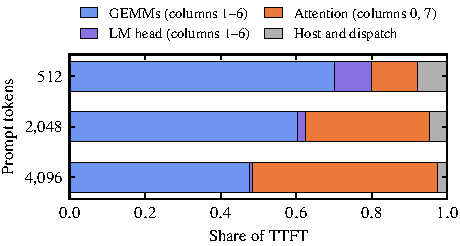
\includegraphics[width=\linewidth]{fig/busy.pdf}
    % VALUE: in the existing prefill, attention's share grows with prompt length, and each column group idles while the other computes
    \caption{Share of time-to-first-token (TTFT) of the existing Llama-3.2-1B prefill by prompt length. Device-busy parts are each operator's time when dispatched alone, less the dispatch floor, summed over the prefill.}
    \label{fig:busy}
\end{figure}

% VALUE: the existing expert prefill already places GEMMs and attention on disjoint columns in one configuration, so its operators differ only in their instruction streams; it runs a layer stage by stage with host work between commands
Prefill processes a prompt to produce the first output token, and its latency is the time-to-first-token (TTFT).
Each decoder layer applies a QKV projection, attention, an output projection, and a gated feed-forward network of gate, up, and down projections.
The open expert prefill of MLIR-AIR~\cite{wang2026mlirair}, laid out like that of FastFlowLM~\cite{fastflowlm-repo}, places every operator of a layer in one configuration, with the GEMMs on columns 1--6 (24 cores) and attention on columns 0 and 7 (one group of 4 cores per column).
Its cores loop indefinitely and take their work from runtime parameters, so its operators differ only in their instruction streams, and each command keeps only the instructions for its own operator's columns.
The prompt is processed in chunks of 128 tokens, and the host runs a layer stage by stage: the QKV projections of all chunks, then each chunk's attention, then each chunk's remaining projections.
The host CPU computes the normalizations, the rotary position embedding, and the residual additions between commands.
% SOURCE: mlir-air a3e26261 programming_examples/llms/shared/fused_prefill/: device.py (column map cols(cfg); "one PDI serves every op and shape and the ops differ only in their insts"), engine.py (strip_columns), dense.py (_mix_all, stage-major order), hostops.py.

% VALUE: the existing prefill issues one operator per command, so its column groups take turns; attention's growing share is time the GEMM columns sit idle
The existing prefill issues one operator per command, which amounts to about 1{,}500 commands for a 2{,}048-token prompt.
Figure~\ref{fig:busy} shows the resulting split of TTFT: device-busy time accounts for 92--97\% of it, and attention's share grows from 12\% to 49\% between 512 and 4{,}096 tokens.
Because the commands run in submission order, columns 1--6 idle while attention runs, and columns 0 and 7 idle while the GEMMs run.
% SOURCE: commands = 16 layers x chunks x 6 + 11 LM-head commands = 1,547 at 2,048 tokens (lab-prefill-census (1)).
% SOURCE: amd-npu e3acc8a prefill-e2/decomp.txt via figs/make_figs.py: busy = isolated time - dispatch floor = 92/95/97% of TTFT at 512/2k/4k; of TTFT, attention 12.2/32.9/49.1%, GEMMs 70.1/60.3/47.6%, LM head 9.7/2.1/0.8%.
% SOURCE: serial execution, the isolated busy times sum to at most TTFT (lab-prefill-device (4)); queued commands do not overlap (Section 3).

% VALUE: packing operators into one dispatch is standard practice for amortizing host overhead; on an in-order CP it does not by itself create concurrency
Placing several operators in one dispatch to amortize per-dispatch overhead is standard practice, as in CUDA Graphs~\cite{nvidia-cudagraphs}, XRT's run lists~\cite{xrt-repo}, and the multi-launch programs that MLIR-AIR stitches together~\cite{wang2026mlirair}.
On the NPU, operators in one command still execute in the CP's instruction order.
Packing therefore removes dispatch cost but creates no overlap unless the operators occupy disjoint columns and the CP issues each one's work before it waits on another's (Section~\ref{subsec:semantics}).
% SOURCE: XRT run list, /opt/xilinx/xrt/include/xrt/experimental/xrt_kernel.h:21 (XRT 2.25.0); MLIR-AIR stitch_elf (vault src-mlir-air-llms).

\subsection{Related Work}
\label{subsec:related}

\textbf{Mapping and Fusion on Spatial Accelerators.}
% VALUE: mapping frameworks choose fused groups and their placement; the designs are separately issued, and their concurrency is not addressed
Stream explores layer-fused mappings on multi-core dataflow accelerators with memory- and communication-aware cost models, and its AIE backend emits one design per fused group~\cite{symons2025stream}.
MLIR-AIR and IRON compile operators and fused multi-operator designs onto the AIE array~\cite{wang2026mlirair,hunhoff2025iron}.
These works decide what a design computes and where, whereas our setting takes the designs as given and concerns how one CP issues them.
% SOURCE: Stream describes no switching cost and no concurrency across fused groups (vault src-stream-dse, arXiv v2 read 2026-10-14).

\textbf{Concurrent Operators on GPUs.}
% VALUE: GPU serving overlaps heterogeneous operators within one device, where the hardware schedules concurrent kernels
NanoFlow splits a batch into nano-batches so that compute-, memory-, and network-bound operations overlap within one GPU~\cite{zhu2025nanoflow}.
On a GPU, kernels on separate streams are scheduled concurrently by the hardware, whereas on the NPU, concurrency must be written into one in-order instruction stream.
% DECISION: the NanoFlow sentence states only what its paper shows; read the PDF and add a vault source note before submission.

\textbf{LLM Inference on AMD NPUs.}
% VALUE: existing NPU LLM runtimes compose hand-tuned designs per model, with the composition fixed by hand
FastFlowLM runs many model families on XDNA~2 NPUs with hand-tuned designs~\cite{fastflowlm-repo}, and MLIR-AIR builds end-to-end decoder models from fused operator designs~\cite{wang2026mlirair}.
In both, the composition of operators into commands is fixed by hand for each model, whereas our setting derives it from the designs' instruction streams.

\textbf{Scheduling with a Shared Server.}
% VALUE: classical scheduling covers machines that share one server and reentrant shops; the CP is a server that also blocks on completions
Scheduling theory studies parallel machines whose jobs each need a common server for setup~\cite{hall2000common,glass2000dedicated}, and reentrant shops in which jobs return to a machine several times~\cite{wang1997reentrant}.
The CP resembles such a server, with the difference that it also blocks on synchronizations until a machine's work completes.
% DECISION: these three works are cited from their metadata only; read each PDF and add a vault source note before submission.

\section{The Order Is in the Program}
\label{sec:order}

% VALUE: on XDNA 2 each engine runs its program in order and nothing schedules across engines, so the order of the work and the waits between engines are in the compiled program; the section shows this from measured command semantics, states the execution model, reads a stream into a happens-before graph with a cause per wait, and extends the reading to closed binaries
On XDNA~2, each engine runs its own program in order, and no hardware or runtime scheduler reorders work across engines, while arbitration on shared ports and locks serializes work at run time and enters the analysis as a resource.
The order of the work and the waits between engines are therefore fixed by the compiled program and the host's dispatch sequence, whereas their durations are not.
We first establish how the CP turns instruction streams into concurrency (Section~\ref{subsec:semantics}), then state the execution model the analysis assumes (Section~\ref{subsec:model}), read a stream into a graph of what must finish before what starts, with a cause for each wait (Section~\ref{subsec:reading}), and extend the reading to binaries shipped without source (Section~\ref{subsec:closed}).

\subsection{Command Semantics}
\label{subsec:semantics}

% VALUE: the CP semantics, measured on the existing prefill's own operators, say where concurrency can come from: not from queued commands, but from one command that issues both groups' work before it waits on either
To find where concurrency can come from, we measure how the CP turns instruction streams into overlap on the existing prefill's own operators, pairing one attention operator on columns 0 and 7 with one GEMM operator on columns 1--6.
Every composed command here produces outputs bit-identical to those of the operators run alone.

\begin{figure}[t]
    \centering
    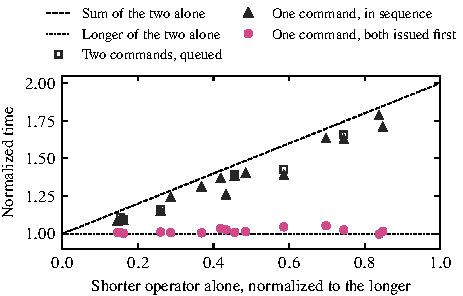
\includegraphics[width=\linewidth]{fig/pairs.pdf}
    % VALUE: queued commands take the sum of the two operators, one command that issues both before waiting takes the longer one
    \caption{Median time of one attention and one GEMM operator on disjoint column groups, normalized to the longer operator alone, over 20 runs per pair. Holding both streams in one command saves one dispatch floor against the sum.}
    \label{fig:pairs}
\end{figure}

\textbf{Queued Commands.}
% VALUE: the runtime gives no overlap across commands, and placing two operators in one command is itself neutral, so overlap must come from within a command
Two commands queued on one hardware context, with no wait between them, take as long as one command that holds both streams in sequence, within 3\% on every pair (Figure~\ref{fig:pairs}).
Holding both streams in sequence in one command takes the sum of the two operators' times minus one dispatch floor, within 2\%, so placing two operators in one command is itself neutral.
This is why packing several operators into one dispatch, which is standard practice for amortizing launch cost, as in CUDA Graphs~\citep{nvidia-cudagraphs}, XRT's run lists~\citep{xrt-repo}, and MLIR-AIR's multi-launch programs~\citep{wang2026mlirair}, removes dispatch cost on the NPU but creates no overlap.
% SOURCE: queued / in-sequence = 1.007-1.029 on 7 pairs (amd-npu 17f7ec3 prefill-overlap/ovl4/, lab-prefill-overlap (5)b); in-sequence / (A + G - F) = 0.996-1.021 over 17 pair runs (ovl/, ovl2/ at 8f13e05 and ovl4/; report.txt H1 column).
% SOURCE: XRT run list, /opt/xilinx/xrt/include/xrt/experimental/xrt_kernel.h:21 (XRT 2.25.0); MLIR-AIR stitch_elf (vault src-mlir-air-llms).

\textbf{Concurrent Issue.}
% VALUE: one command that issues both groups' work before it waits on either runs them concurrently at nearly the longer one's time; the small cost appears when both read DRAM near the cap
When one command issues all of the GEMM's work, then the attention operator's stream, and only then the GEMM's synchronizations, the two operators run concurrently.
Such a command takes 1.00--1.06 times the longer operator's time on 9 pairs that cover three GEMM shapes and attention over chunks 0 to 15 (Figure~\ref{fig:pairs}).
On six further pairs with other shapes and chunks, the overlap hides 90--96\% of the shorter operator's work, after excluding the dispatch floor that the merge already saves.
The overlap costs most when the pair's combined DRAM read rate approaches the read cap, at about 95\% of the cap measured in the same batch.
The serial execution of the existing prefill is therefore a property of how its commands are composed, not of the array or its configuration.
% SOURCE: interleaved / max(A, G) = 0.998-1.058 over 10 pair runs = 9 pairs (c8 + lm measured twice, 1.054 and 1.058; the figure keeps each pair's first measurement); GEMM shapes up, LM head chunk, down; attention chunks 0, 4, 8, 12, 15 (lab-prefill-overlap (3)).
% SOURCE: hidden fraction of the shorter operator's work, (in-sequence - interleaved) / (min(A, G) - F) = 0.90-0.96 on 2+qkv, 6+o, 11+gate, 14+qkv, 6+gate, 11+o (lab-prefill-overlap (5)a).
% SOURCE: DRAM rate during the interleaved command 52.2 GB/s against a same-batch 8x2 cap of 53.9-55.3 GB/s for c8 + lm, the costliest overlap (1.054-1.058) (lab-prefill-overlap (3)).

\textbf{Synchronization Order.}
% VALUE: because the CP is in order, a wait on one group delays the issue of every other group's work; the attention measurement of Section 4.1 isolates this effect, so the instruction order is a scheduling decision of its own
Since the CP executes in order, a synchronization on one group delays every later issue, including the issue of another group's work.
The existing attention operator isolates this effect (Section~\ref{subsec:losses}): its two columns carry equal work, yet alternating their segments lowers its device time to $0.67\times$ at 2{,}048 tokens with the same instructions.
The CP's instruction order, and not only the assignment of operators to commands, is therefore a scheduling decision.
% SOURCE: vault lab-prefill-overlap (4)-(5)c; Section 4.1 carries the numbers.

\textbf{Hardware Contexts.}
% VALUE: a second hardware context gives no concurrency here: the driver's source allocates every context the whole array and shares it in time, and narrower partitions would need contiguous columns, rebuilt designs, and a host round trip at every dependence, so concurrency comes from within one command
Two hardware contexts on disjoint partitions are the obvious alternative, but the driver's source shows that every hardware context on our platform is allocated all eight columns, so co-resident contexts share one partition in time.
Even where narrower partitions are allowed, a partition spans contiguous columns, whereas the existing attention sits on columns 0 and 7, so each group would need its own rebuilt design.
Every dependence between attention and a GEMM would then cross the host, which waits on one context before it submits to the other.
Concurrency on the array therefore comes from within one command, which needs no rebuild and no change to the driver or firmware.
% SOURCE: amdxdna 2.25.0 (loaded module 2.25.0_20260922, NPU Strix Halo 1022:17f0 rev 11, firmware 1.1.2.65): every firmware protocol the driver accepts on this device enables AIE2_TEMPORAL_ONLY (npu4_regs.c:94-106, the table npu5 shares), and aie2_alloc_resource (aie2_ctx.c:604-608) then requests start column 0 and all columns for every context, which the solver shares as one partition (vault lab-prefill-overlap (31)).
% SOURCE: contiguous partitions, separate 6- and 2-column builds with attention moved onto adjacent columns, and the host round trip (vault lab-prefill-overlap (1)).
% DECISION: the temporal sharing is stated from the driver's source with the driver named; a two-context behavioural check is registered and not run, so it is never worded as a measurement.

\subsection{Execution Model}
\label{subsec:model}

% VALUE: the analysis models a dispatch as operations on engines (CP instructions, BD executions, core loop iterations), each with read and write sets over locations that include every exclusively held resource; under static control one dispatch at given runtime parameters has one static set of operations, a loop with data-dependent control is reported and left out, and durations stay measured inputs
The analysis models a dispatch as operations on engines, each with a set of locations that it reads and a set that it writes.
A command contributes one operation per instruction of its stream on the CP, a DMA engine one per execution of a BD on one channel, and a core one per iteration of each counted loop.
Locations cover every resource that one operation holds exclusively, namely bytes of DRAM, memory tiles, and local memory, as well as BD slots, locks, DMA channels, task-queue slots, stream-switch ports, and configuration registers, so a structural hazard is also a conflict on a location.
For example, a lock acquire reads and writes its lock, a queue push writes a queue slot and reads its BDs, and a BD execution reads its BD slot and its source bytes and writes its destination bytes.
We assume static control: the CP's stream is straight-line, since a synchronization waits but does not branch, and every core loop is counted, with a trip count that depends on the dispatch's runtime parameters rather than on computed data.
A dispatch at given runtime parameters then has one static set of operations, and a loop with data-dependent control is reported as such and left out of the analysis.
A loop whose body holds nested control, or an access the analysis cannot classify, is likewise reported as unsupported and not analysed, which in the decode design applies to every loop outside attention.
We also assume that the host follows static control, issuing commands in an order that depends on the LLM and the lengths of the context and the prompt rather than on data, and its own work enters as a measured cost.
Durations remain measured inputs, because the program fixes the order of each engine's work but not how long the work takes \E{the per-operation costs from the microbenchmarks}.
% SOURCE: operations, locations, and static control (vault lab-cosched-passes (30), item 1); unsupported loops: 22 in the decode census build, all outside the attention herd (lab-cosched-passes (33), Limits); the host's static control (outline v9 section 1); the decode kernels' early return on the pad block branches on a runtime parameter, so it stays static per context length (lab-decode-long-context (10)).

\subsection{Reading a Stream}
\label{subsec:reading}

\begin{table}[t]
    \centering
    \caption{Ordering Mechanisms}
    \label{tab:mech}
    % VALUE: the 11 mechanisms that create a direct happens-before edge, in attribution order, with the granularity of each
    \begin{tabular*}{\linewidth}{@{\extracolsep{\fill}}rlr}
        \toprule
        \# & Mechanism & Granularity \\
        \midrule
        1 & CP synchronization and mask-poll & stream \\
        2 & CP in-order issue (completes at issue) & stream \\
        3 & Channel task queue (FIFO, depth 4) & stream \\
        4 & Dispatch order on one context & stream \\
        5 & Configuration and control-packet writes & stream \\
        6 & BD chaining and repeat & data movement \\
        7 & Locks on DMA BDs & data movement \\
        8 & Stream-switch back-pressure & data movement \\
        9 & Cascade and neighbor memory & data movement \\
        10 & Core locks & core loop \\
        11 & Core program order & core loop \\
        \bottomrule
    \end{tabular*}
\end{table}

% VALUE: happens-before is completion before start, not issue order; each direct edge comes from one of 11 mechanisms at the stream, data-movement, or loop granularity and is attributed to exactly one, and edges no mechanism explains are counted, so the count measures the model's coverage
From these operations, the analysis builds a \emph{happens-before} graph, in which an edge from $a$ to $b$ means that $b$ cannot start until $a$ has completed.
Issue order alone does not create such an edge, because a queue push is issued in order but its transfer completes later.
Each direct edge comes from one of the 11 ordering mechanisms of Table~\ref{tab:mech}, at the granularity of the CP's stream, of data movement, or of a core loop, and an edge that two mechanisms imply is attributed to the first in the table.
An operation whose ordering effect no mechanism describes, such as an unknown opcode or a write outside the known register map, takes edges to its neighbors on the CP, and counting these per stream is how the model's coverage is to be measured.
Edges of mechanism 2 never stall, because their instructions complete at issue, so they are attributed but reported apart from the blocking edges.
% SOURCE: the mechanism table, attribution order, granularities, UNATTRIBUTED, and issue edges (vault lab-cosched-passes (30), item 2); the library AIECoschedDeps (mlir-aie f1725dae1f1, pinned).

% VALUE: each direct edge is classed by the pairs of operations it alone orders: a true dependence if one is read after write, a name dependence if one is write after read or write, an order dependence otherwise; classes say whether renaming or reordering can remove the wait; a wait gating several operations is classed per gated operation, pairs ordered by two disjoint paths are counted as redundant, and data-dependent loops as control
For each direct edge, the analysis computes the pairs of operations that the edge alone orders, namely those ordered with it and not without it.
The edge is a true dependence if one of these pairs reads a location after the other writes it, a name dependence if none does but one writes after the other reads or writes, and an order dependence otherwise.
The first two follow the conflicts that Bernstein's conditions exclude between pieces of work that run in parallel~\citep{bernstein1966analysis}, and the name class covers the anti and output dependences of compilers~\citep{kuck1981dependence}.
Renaming the conflicting locations can therefore remove a name dependence, reordering can remove an order dependence, and a true dependence stays.
A synchronization that gates several operations contributes one edge per gated operation, so each operation's conflicts are classed on their own.
A pair that two disjoint paths order is lost by no single edge, so each edge on those paths may be classed as an order dependence alone, and such pairs are counted as redundant instead of being attributed to either path.
A loop with data-dependent control is counted as control.
% DECISION: this subsection states the classification the passes assume and the counts it defines, not what the committed library computes. Verified against mlir-aie f1725dae1f1 on 2026-10-21: AIECoschedDeps classifies each core loop's buffers and reports its lock edges and loop-carried distances, so the class of a wait at loop granularity is computed; the edge-level attribution, the unattributed and redundant counters, and the order class itself are not implemented there, and the order class is unreachable in that library. The stream-granularity instances this paper removes were identified by reading the designs and confirmed by measurement, and the graph of a compiled stream is built by the prefill reader rather than by the library. Every sentence here is written in that register until the attribution pass exists. The registered census of Section~\ref{subsec:census} is a DIFFERENT quantity and does not depend on this: it counts instances that the frozen scheduling pass proposes, removes and confirms, and it never classifies edges. The coverage counters owed with the attribution pass are the unattributed and redundant counts, which were never part of that census (pass-0, 2026-10-22).
Loop-carried edges are classed in the same way on the loop's iterations, with their distance recorded.
% SOURCE: classification by Lost(e), REDUNDANT, CONTROL, loop-carried distance (vault lab-cosched-passes (30), item 3).

% VALUE: the recovered order is the method and is checked through its consequences, not against a trace: removed false waits leave outputs bit-identical, measured gains stay within their bounds, and what the analysis leaves out is counted; the CP's own timer records show the issue and wait order inside each command without changing the array's configuration, and they cannot see core loops or the gaps between commands
We check the recovered order through its consequences rather than against a hardware trace.
Every wait that the analysis classes as false and that our passes remove leaves the outputs bit-identical (Section~\ref{sec:method}), each measured gain is compared with its bound (Section~\ref{subsec:tests}), and the operations that the analysis leaves out are counted per stream.
To show how the CP executes the order, we insert the runtime's record-timer instruction after each synchronization and after each run of issue instructions, so that the firmware writes an identifier and a 1.8~GHz device timer into a buffer that the host reads after the run.
The array's configuration is left unchanged.
On one 128-token prefill chunk of Llama-3.2-1B, 1{,}468 records per run leave the logits bit-identical and add no measurable device time.
For each command, they show when each column group's work was issued and how long each synchronization blocked the CP (Figure~\E{timeline}).
Between commands the timer advances at less than a tenth of its rate, so the records time intervals within a command, whereas the host's clock times the gaps between commands.
Order inside a core's loop is invisible to the CP, so the decode loop's order rests on its removal (Section~\ref{subsec:rings}).
% SOURCE: record-timer instruction TXN opcode 0x83 (12 bytes: header, size, 32-bit id; aiebu 48b69735 xaie_txn.h), XRT 2.25.0 ML Timeline (XDP 67165d6 clientDev/ml_timeline.cpp; Strix Halo listed as a client device with a debug buffer); feasibility check: split-1b-S4-L20480, 108 commands, 1,468 records per run, 5 runs with and 5 without, logits sha equal in all 10, summed start-to-wait with / without records 0.93-0.95, per-command fit of the timer 1,752-1,767 MHz against the 1,800 MHz H clock at the top DPM level (xdna-driver bc5dd96 npu4_dpm_clk_table), 110-125 M timer cycles per host second between commands (amd-npu b98e3044; vault lab-flm-streams (39), decisions log D13).
% DECISION: T-rec was withdrawn by the author (outline v9 revision 31, D13); recovery is the method in every verb row, and the timer records are a figure that governs no verb.

\subsection{Closed Binaries}
\label{subsec:closed}

% VALUE: a closed stack ships binaries only, so its streams are recorded at the runtime's boundary without the device and lifted with a byte-identical round trip; each issue is attributed to the column group its data reaches through the configuration's decoded routes; FastFlowLM's prefill then issues one group per command, and serial issue predicts its time where overlap does not
FastFlowLM ships its engines as binaries, so we record their instruction streams at the runtime's boundary, either with a recording library that never opens the device or with an interposer during a device run, and lift each stream into MLIR-AIE's runtime-sequence form.
Every stream recorded offline round-trips through the lifter byte for byte, so the analysis reads exactly what the engine dispatches.
Because FastFlowLM's attention reads through shim tiles of the GEMM columns, attributing an issue to its column would mix the groups, so the analysis decodes the configuration's stream routes and attributes each issue to the group whose compute tiles its data reaches.
Under this attribution, the one capture we analyse, a 1{,}009-token prefill of Gemma-4-E2B, changes column group only at the boundary between two commands, once into attention and once out of it in every layer, so it issues serially, one group per command.
The sum of its commands' times measured alone, each less the dispatch floor and plus the boundary cost between commands, matches its measured time within 10.0\%, inside the check's tolerance of 20.8\%, whereas full overlap would place it 36.5\% lower.
A census of which columns carry any instruction, over all 218 recorded streams and over the capture itself, agrees with this attribution without establishing it, since it counts addressed columns rather than the programs they serve; Appendix~A gives the counts.
Since FastFlowLM's closed libraries build these streams and their buffers, we measure removals on MLIR-AIR's fused prefill, which reimplements FastFlowLM's designs~\citep{wang2026mlirair}.
Its decoded configuration places the GEMMs on columns 1--6 and attention on columns 0 and 7, as FastFlowLM's fused prefill does, so the two share the column groups whose turns our passes remove.
Appendix~A states how the attribution was chosen, and what the rule registered before it labels the same capture.
% SOURCE: recording libhrx (FastFlowLM 44d01787, gemma4e-flash), every prompt length 1-1,024 recorded with 0 /dev/accel opens; 8 buckets, 218 distinct streams, round trip and identity 218 / 218 (vault lab-cosched-passes (14)); lifter fix mlir-aie 91f64387ffb, 375 / 375 MLIR-AIR streams byte-identical (lab-cosched-passes (3)).
% SOURCE: device capture through an XRT interposer, gemma4e-flash:e2b, 1,009 tokens; route maps from the frozen cdo_routes decoder: shim 3 and shim 6 MM2S0 reach only columns 0 and 7; 70 group transitions, all between commands (35 GEMM -> attention, 35 attention -> GEMM) (vault lab-flm-streams (11), (13)).
% SOURCE: ops-per-column census over the 218 FLM streams, recomputed here from the committed artifact (aie-cosched 0400fc9 passes/results/bprime/column_ops.json, from bprime_column_ops.py 879bf80; parsed by aie-cosched-pass-0, counts re-derived independently in this workspace): column sets {1,2,3,4,5,6} 200, {0,3} 8, {6,7} 8, {} 1, all eight 1. Every {0,3} stream carries the bulk of its ops on column 0 (e.g. 1,420 against 384) and every {6,7} on column 7, which matches the frozen route map above (shim 3 and shim 6 MM2S0 reach only columns 0 and 7), so the 16 are attention commands plus their feeding shim. The peer's first message said 192 of 218 and corrected it to 200; 192 is the count among proposal streams only. The one empty stream (186fd90831c87d8c) was earlier reported as "not analysed: one column" and in fact has no ops.
% SOURCE: closed-stack check: T = 1.444 s, serial prediction 1.300 s (error 0.100), overlap prediction 0.917 s (error 0.365), tolerance 0.2075, of which 0.102 is one slow floor repetition; without it the tolerance is 0.106 and the serial prediction still passes (vault lab-flm-streams (12) RESULT, amd-npu 52c8401d, 3d0d1036).
% SOURCE: MLIR-AIR's llms README: "reimplement AMD NPU LLM designs originally developed by the FastFlowLM team" (mlir-air 740cae0f, a3e26261); fused_prefill/device.py "laid out like FastFlowLM's fused_prefill"; FastFlowLM's Gemma4-E2B fused_prefill.xclbin decoded with tools/xclbin_layout.py: attention programs on columns 0 and 7, a GEMM program on the 24 cores of columns 1-6 (vault lab-flm-streams (5)); coverage ruling D13(b).
% DECISION: the serial label is scoped to this one capture (Gemma-4-E2B, 1,009 tokens, the engine's cap); the attribution by routes was ruled after the capture, and the label under the first attribution by tile column was MIXED-majority; both disclosures go to the appendix (outline v9 section 2, C2).

\section{Scheduling Passes}
\label{sec:method}

% VALUE: the passes and their legality checkers are the implementation: the composer reorders and renames across the operators of the open prefill, the stream pass reorders within one operator's stream, the loop pass renames inside decode attention's loop, and each output is checked for legality from the instructions and run bit-identically; the event model makes each choice before anything runs
Our passes remove false dependences of the classes of Section~\ref{subsec:grid}, and legality checkers accept each rewrite before it runs.
In decode's loop the class and the buffers come from the analysis of Section~\ref{subsec:reading}; in the CP's stream they were identified by reading the designs, and the analysis supplies the graph against which each rewrite is checked.
For the open prefill, a composer takes an existing design's per-operator instruction streams, its map of operators to columns, the dependency graph of its host program, and the probes, and emits a sequence of composed commands.
The composed commands must do the same work as the existing ones, which the composer guarantees by keeping every instruction and checking legality from the instructions themselves (Section~\ref{subsec:compose}).
No group may wait at the CP for work it does not consume, which is an order dependence in the stream row of Table~\ref{tab:grid}, so the composer reorders issue across operators and a stream pass reorders issue within one operator's stream (Section~\ref{subsec:order}).
No use of a buffer may wait for another use it does not depend on, which is a name dependence in the same table, so the composer renames buffers into rings and our loop pass renames decode attention's buffers by the same rule (Section~\ref{subsec:rings}).
The partition of the array must fit the regime, so the composer chooses the split of columns for each regime (Section~\ref{subsec:split}).
The event model of Section~\ref{subsec:pricing} prices every candidate, so each choice is made without running the candidate.
Removing a dependence is not always worth its cost, and Section~\ref{subsec:removal} gives both the rule that decides and the regime where the composed order loses time.
% SOURCE: amd-npu a0ee2edf44e0 (tag composer-v1.1), prefill-overlap/txn.py, merged.py, component_model.py; Python, on the engine's hardware context; the stream pass aie-cosched-schedule and the loop pass aie-cosched-rename in mlir-aie (aie-cosched-pass-0 f1725dae1f1).

\subsection{Composing Instruction Streams}
\label{subsec:compose}

% VALUE: a composed command is an interleaving of operators' segments that keeps each operator's own order and every instruction once, so only the timing of issue and waits changes
The composer splits each operator's instruction stream, already reduced to its own columns, into the segments of Section~\ref{subsec:formulation}.
A composed command concatenates segments of several operators in a chosen order, keeping each operator's segments in their own order and every instruction exactly once.
Under these rules, an interleaving changes only when each operator's work is issued and awaited, never what the work is.
% SOURCE: txn.segments and txn.compose (amd-npu a0ee2ed prefill-overlap/txn.py); compose asserts each stream's segment order, every op kept once, and equal headers.

% VALUE: two operators may interleave only if they cannot disturb each other's device state, which the composer checks statically from the instructions themselves; operators on one group stay in sequence
Two operators may interleave in one command only if they cannot disturb each other's state on the device, which the composer checks from the instructions themselves.
Every register write of an operator must address a column of its own group and touch only shim BDs and DMA queues, the operator's own cores' locks, and runtime parameters in its own cores' memory.
Interleaved operators must patch disjoint argument slots or disjoint byte ranges of one slot's buffer, and no operator may write a buffer that another operator in the same command reads or writes.
Operators on the same group, such as several GEMMs, are composed in sequence rather than interleaved, so their writes to that group's registers keep the order of separate commands.
% SOURCE: each check turns red on a defeated input (swapped groups, an unstripped stream, a synchronization before an issue op, a patch onto another group's argument, a duplicated column, a reordered or dropped segment) (lab-prefill-overlap (3), (4)).

\subsection{Reordering Issue}
\label{subsec:order}

% VALUE: the composer list-schedules the dependency graph chunk by chunk rather than stage by stage, so each attention operator meets independent GEMMs of earlier chunks, and it sizes each command so its GEMM work matches the attention work
The existing host program runs each layer stage by stage, so every output projection waits behind the layer's entire attention, and no GEMM is ready to run beside attention.
The composer instead list-schedules the dependency graph chunk by chunk.
At each step, it takes the ready attention operator of the lowest layer and chunk and adds ready GEMMs, in the same order, until their estimated work reaches that of the attention operator.
The GEMMs then run in sequence on columns 1--6 while attention runs on columns 0 and 7.
% VALUE: the price of running the two groups at once: the columns share the DRAM read cap, so a group whose partner is bandwidth-bound loses a measured share of its partner's time, and the ceiling on a pair is below the ideal; where a group is already near the cap there is nothing to win
Running the two groups at once is not free, because the columns share one DRAM read rate.
A group on the critical path loses 8.5\% of its partner's duration when it is bandwidth-bound and almost nothing when it is not, so two operators of equal duration overlap to within $1.84\times$ of the longer rather than the ideal $2.00\times$ (Section~\ref{subsec:removal}).
Where a design already reads near the cap the reorder therefore has little to recover, which Section~\ref{subsec:bound-eval} reports for the largest model we evaluate.
% SOURCE: the penalty by regime and the 1.84x ceiling are Section 5.1's measurement; per command on Llama-3.2-1B at 4,096 tokens, commands carrying GEMMs read 90-93% of the cap and commands carrying attention about 15% (vault decisions log, "Regime analysis" steps 1 and 3); the 8B composed prefill averages 93-96% of the cap (lab-metric-fields (1)).
% DECISION: tradeoffs are stated beside the decision that incurs them rather than collected in a section (author, 2026-10-21).
For an append to a cached context, the composer plans only the new chunks, and their attention estimates use each chunk's absolute index.
% SOURCE: merged.plan (a0ee2ed): qkv(L, c) after down(L-1, c); attn(L, c) after qkv(L, 0..c); o after attn; gate and up after o; down after gate and up; an optional cap on the GEMMs per attention command.
% SOURCE: append = Merged.prefill(ids, start=L) on the same plan rules; attention estimates linear in the absolute chunk index (vault lab-agent-step (1)).

% VALUE: within a command, the CP opens every group's work first and then places each synchronization at its predicted completion, followed by the issue it gates, so no synchronization holds back another group's work; the order is fixed before dispatch from the estimates
Within a command, the order of synchronizations decides how long each group waits for its next issue (Figure~\ref{fig:order}).
In turn, the CP would issue the first GEMM, then walk the attention stream to its end, and only then issue the second GEMM, so the GEMM group idles behind attention's synchronizations.
The composer instead issues the opening segments of both attention columns and of the first GEMM, and then places every synchronization in order of its \emph{predicted completion}, each followed by the issue it gates.
A GEMM's synchronizations are predicted to complete after the sum of the estimates of the GEMMs before it, and attention's mid-stream synchronizations at fixed fractions of its estimate.
Attention's two columns are treated as two groups, so their segments alternate, which removes the false dependence inside the attention operator (Section~\ref{subsec:losses}).
The order is static: the estimates fix it when the command is built, and the device executes it without host involvement.
When issue costs are negligible, the estimates are exact, and the host work is hidden, the CP never blocks on a later-completing operator while an earlier one's successor waits, so the order matches the list schedule of the groups without a CP.
% SOURCE: merged.cp_order (a0ee2ed); mid-stream fractions (0.25, 0.5) of attention's estimate, the lowest of five placements tried; the in-turn order takes 1.26x as long on the same 38 commands (lab-prefill-overlap (16)).
% DECISION: the exactness statement in the last sentence is argued, not proven; it stays a remark until a proof is written (vault ch3-formulation, Lower bound and heuristic).

% VALUE: within one operator's stream, the stream pass's full mode interleaves the columns' segments round-robin by index, the rule that produced the hand-alternated streams, so it emits the alternation byte-identically on the population's attention streams, and the legality checker accepts each rewrite by checking every inverted pair against the decoded configuration
Within one operator's stream, a stream pass on the lifted runtime sequence reorders issue as well.
In its full mode, it interleaves the columns' segments round-robin by index, which is how the alternated attention streams were produced by hand, so it emits that alternation rather than discovering it.
On all 42 attention streams of the population, the pass's output is byte-identical to the hand-alternated stream.
Reproducing a hand edit is the point rather than the limit: a hand edit reaches the streams someone reads, whereas a pass that must accept or refuse every stream has to carry the condition under which the rewrite is legal, which is what lets it reach the streams nobody has read.
A legality checker accepts each rewrite before it runs, by checking every pair of instructions that the rewrite inverts against the routes, BDs, and buffer ranges decoded from the configuration.
% SOURCE: aie-cosched-schedule (mlir-aie 573e0140174, identical in f1725dae1f1), proposal format /2 frozen at aie-cosched 8dee63f; 42 / 42 decoded order and bytes equal to the hand versions (vault lab-cosched-passes (35), (40)); the pairwise inversion rule of legality.py (lab-cosched-passes (14)).
% DECISION: the pass emits the alternation and the checker accepts it; it is never said to discover it, and full mode is never called a predicted-completion rule (Ruling D3, vault decisions log).

\subsection{Renaming Buffers}
\label{subsec:rings}

% VALUE: with commands in flight and chunks interleaved, two uses of one buffer would wait on each other although neither consumes the other's data; the composer gives each overlapping use its own slot, with ring depths derived from the plan's live intervals and a check that no slot is reused before its reader is done
Once operators of several chunks are in flight, a GEMM's input and output buffers cannot be reused per stage as in the existing host program, because two uses of one buffer would then wait on each other.
For each buffer role, the composer derives a ring of slots from the plan: each use of a buffer lives from its producer's write to its last reader's completion, and interval colouring assigns slots so that no two overlapping uses share one.
A separate check asserts, over the whole plan, that no slot is reused before its previous reader has completed.
The depths follow from the plan and are not set by hand; for example, every QKV input of a layer is written before the layer's first QKV command completes, so that ring needs one slot per chunk.
% VALUE: the price of the rings: slots are memory, and the composer buys overlap with it; the arenas replace the engine's own weight buffers rather than adding to them, so the cost is the schedule's slots and not a second copy of the weights
Slots are memory, so this is where the composed schedule pays for its overlap.
The rings and the plan's own buffers take 53--179\,MB across the configurations we build, whereas the arenas that hold the weights replace the engine's own weight buffers rather than adding to them, so the weights are not copied twice.
Peak live device memory for a 4{,}096-token append to a 16{,}384-token context is then 3.5\,GB on Llama-3.2-1B, 7.7\,GB on Qwen3-4B, and 9.7\,GB on Llama-3.1-8B; the production engine holds 2.2 and 7.9\,GB for the first two on the same weights, so the schedule's slots and not a second copy of the weights are what we add.
% SOURCE: composer schedule buffers (Layout plus lazy) 53.4-178.8 MB over the 21 configurations (min 1B S4 16k + 4k, max 8B S2 scratch 2k; amd-npu 71901c50 metrics/retro-2026-10-21/footprint-summary.txt, re-derived in the 2026-10-22 foundation audit); weight arenas 645 MB (1B), 2,340 (Qwen3-4B), 4,451 (8B), replacing rather than duplicating the engine's weight buffers, with peak minus live equal to the arena size within 2% at load; peak live 2,206 / 5,923 / 7,399 MB at 4,096 tokens from scratch and 3,471 / 7,725 / 9,721 MB at 16,384 + 4,096; FastFlowLM's server at drm-total-memory 2,110,100 KiB (1B) and 7,668,316 KiB (Qwen3-4B), i.e. 2.16 and 7.85 GB (mapped 2,158,084,096 and 7,847,751,680 B; the earlier 2.11 / 7.67 read KiB as kB) (vault lab-metric-fields (1); lab-flm-practice (3)).
% DECISION: the tradeoffs are stated beside the decision that incurs them rather than collected in a section (author, 2026-10-21).
% SOURCE: merged.colour, assert_no_hazard, and Layout (a0ee2ed); the hazard check turns red on an overlapping slot; ring depths at 4,096 tokens: shared 2048-wide input 32, 8192-wide input 4, outputs 4-18 (lab-prefill-overlap (9)).

% VALUE: decode attention holds the same false dependence inside one operator: one buffer each for a block's keys, values, and scores makes each block wait for the previous one; renaming alone gains nothing while the scores are acquired once per pair of blocks, as in a hand edit unrolled by two, because the two cores still wait for each other; our loop pass renames all three into two-slot rings acquired once per block on both ends, keeps the carried state, and matches a hand edit's gain with unchanged kernels and bit-identical outputs
Decode attention holds the same false dependence inside one operator, where a single KV buffer makes each block's transfer wait for the compute on the previous block (Section~\ref{subsec:losses}).
Only the running maximum and the accumulator must carry across blocks, whereas each block's keys, values, and scores are written once and read once, so a second buffer for each lets transfer and compute alternate between them.
Renaming alone is not enough, however, when the scores are acquired once per pair of blocks, as in a hand edit that unrolls the loop by two.
With the keys, values, and scores renamed but the scores acquired per pair, the time per token stays within 2\% of the existing design's, since the core that computes a block's scores and the core that folds them into the output still wait for each other.
Our loop pass therefore renames each such buffer into a ring of two slots that each core acquires and releases once per block, so the first core computes block $b+1$ while the second folds block $b$.
The compiler's double-buffering transformation declines the loop because of the carried state, whereas our pass classes every buffer of the lowered loop by its conflicts across iterations and leaves the carried state in place; the kernels and the arithmetic order are unchanged, and the decoded tokens and logits stay bit-identical.
On both models, the pass's output comes within 1\% of a hand edit that passes the scores between the cores through a channel instead, at every evaluated length.
% SOURCE: renamed K, V, and score in the hand edit unrolled by two, scores acquired per pair (arm (b)): 0.997-0.984x per token at 4k-32.5k, slope 1.181 vs 1.153 us (Llama-3.2-1B; vault lab-decode-long-context (13), amd-npu aab2aae); the same edit on Llama-3.1-8B 0.990x at both cells (lab-decode-long-context, decode nulls Phase 2). Loop pass (aie-cosched-rename, mlir-aie 41b4947f09e; classes and rings in vault lab-cosched-passes (33)): against the existing design 1.269x at 16,384 and 1.391x at 32,512 (1B), 1.160x at 16,384 and 1.205x at 28,800 (Qwen3-4B); pass / hand edit 0.992-1.004 at every point; slope 0.683 us (1B) against a transfer-only 0.677 us; tokens and every step's logits bit-identical across the existing design, the hand edit, and the pass, 1B P = 0 to 32,517 and Qwen3-4B P = 2,048 to 28,800 (vault lab-decode-long-context (22), amd-npu a6bc94b and 455740b).
% DECISION: the rename is our loop pass's output on the lowered design, not a hand edit; the hand edit appears only as the reference the pass reproduces.

% MOVED from the former limits paragraph: the scope of what these passes touch
Our passes reorder and rename within one configuration of the array and leave every reconfiguration point where the stack put it, so the gains we report hold with those points unchanged and say nothing about moving them.

\subsection{Partitioning per Regime}
\label{subsec:split}

% VALUE: the split of columns between attention and GEMMs is a build-time parameter of the existing design, fixed by hand; the legal splits follow from the heads, each split is a separate configuration built in seconds, and the composer needs only more argument slots to serve it
The existing design fixes the split of columns between attention and the GEMMs by hand: attention groups are listed per column, and the GEMMs take a contiguous block of the remaining columns.
Since each attention group serves an equal share of the KV heads, a model with 8 KV heads admits attention on 1, 2, or 4 columns, with the GEMMs on the other 7, 6, or 4.
We build each split as its own configuration from the unchanged design source, which takes seconds, and each split's outputs are bit-identical to those of the default split.
The composer serves every split with three argument slots per attention group instead of a fixed six, and it checks every GEMM's encoded iteration count and stride against the shim BD's field limits before it uses a split.
% SOURCE: mlir-air a3e26261 fused_prefill/device.py: Attn(col=...) per group in Config.attn, GCOL0, GNC = 1, 6 as module constants; spec() splits kv_heads evenly, so 1, 2, or 4 attention columns with 8 KV heads (vault lab-split-sweep (1)).
% SOURCE: out-of-tree split modules, builds of 13-14 s; logits bit-identical to the default split in every configuration on both models (vault lab-split-sweep (2), (4), (5)).
% SOURCE: BD iteration wrap 6 bits (at most 64 rounds), stride 20 bits (words); the four-column split's LM-head GEMM runs 48 rounds; decoded from aie-rt xaie2pgbl_params.h fields with a round-trip check (vault lab-split-sweep (5)).

% VALUE: the composer picks the split per regime with the event model from one probe per split; more attention columns shorten attention, whose time grows with the context, but lengthen every GEMM, so the choice depends on the prompt and the cached context
For each split, the composer probes every operator alone once and predicts the TTFT of each regime with the event model (Section~\ref{subsec:pricing}), and it picks the split with the lower prediction.
More attention columns shorten attention, whose time grows with the context, but lengthen every GEMM, so the choice depends on the prompt length and on the cached context.
Which group binds the lower bound decides the direction: the GEMMs bind for prompts computed from scratch, so the faster split gives them more columns, whereas attention binds for appends to a long cached context, so the faster split gives attention more (Section~\ref{subsec:bound-eval}).
% SOURCE: per-split probes at n = 2,048, prediction with component_model.simulate (amd-npu 0f61651 prefill-overlap/g1_split_model.py, vault lab-split-sweep (6)-(7)).
% SOURCE: the four-column split's GEMMs are 27% (1B) and 35% (Qwen3-4B) slower than on six columns, and its attention slope per chunk 3.0-3.1x lower than the default split's existing stream (vault lab-split-sweep (4)-(5)).

% VALUE: the chosen splits stay resident, so a conversation switches between them at a turn boundary by a suspend and resume; its cached context, laid out by the attention groups of the split that computed it, moves with it
A deployment keeps each chosen split resident in its own hardware context, with its own copy of the weights, and switches between them at a turn boundary by suspending one context and resuming the other.
The KV cache of a cached context is laid out by the attention groups of the split that computed it, so a conversation that changes split also moves its cache to the new layout.
% VALUE: the price of making the partition a per-regime choice: each split is its own configuration, so a deployment either holds two of them with two copies of the weights or pays a switch and a cache relayout; the weights are the larger of the two costs on a large model
Making the partition a choice therefore costs either memory or a switch.
Each split is its own configuration, so holding both resident holds the weights twice, which on the largest model we evaluate is 4.5\,GB of weight arenas for each; releasing one instead costs a warm switch, 7--8\ms{} on the two smaller models, and the cache relayout above.
Neither cost applies within one regime, where a single split serves every turn.
% SOURCE: weight arenas 645 MB (Llama-3.2-1B), 2,340 (Qwen3-4B), 4,451 (Llama-3.1-8B), one copy per resident split (vault lab-metric-fields (1)); warm switch 7.1 ms (1B) and 7.7 ms (Qwen3-4B), suspend and resume only, without moving a cached context (lab-split-sweep (5)).
Moving the cached context between splits is the cost we do not measure, and it is the one that decides between the two paths.
Its floor, reading and writing the per-block records once at the part's peak memory bandwidth, is 0.6--4.1\,ms on Llama-3.2-1B and 2.7--18.6\,ms on Qwen3-4B over cached contexts of 4{,}096 to 28{,}672 tokens; the closest host operation we have measured, the scatter that seeds a decoder, puts it nearer 26--181\,ms and 116--814\,ms.
On the measured figure the move costs between 4 and 106 times the warm switch, so a deployment that switches regimes often holds both splits resident and pays the memory instead; on the floor alone the smallest model's move would be cheaper than the switch, so we state both and claim neither as the price.
% SOURCE: computed host-only by npu-gap and recorded here: records are layers x kv-heads x ceil(L/32) blocks at 4,608 B (Llama-3.2-1B) and 9,216 B (Qwen3-4B) per block per head, giving 75.5 / 302.0 / 528.5 MB and 339.7 / 1,359.0 / 2,378.2 MB at 4k / 16k / 28k. Floor = 2R at the part's 256 GB/s peak (lscpu, a specification figure, not measured). The nearer figure applies the restack fit's seed term, 342.16 ms per GB written (amd-npu a61417d0 fit-2026-10-21.json), which is an order of magnitude and not a price: it includes a cast a record copy does not do, excludes the per-block sync, and was measured in the clean host state, the same work having fallen into the huge-page excursion of Section 8.1 at 6-14x.
% DECISION: npu-gap's bound contradicted my expectation that the move is an order of magnitude above the switch everywhere; it is not, on the floor at the 1B. Both numbers are stated and neither is called the price.
% SOURCE: switch = suspend + resume + first prefill in one process, both splits' weights resident (vault lab-split-sweep (5)).
% DECISION: the relayout and its decision rule enter once measured (vault paper-cosched-plan, regime switching); until then this sentence stays a placeholder.

% VALUE: what a platform must offer for the method to apply: an in-order issuer whose issue returns at once and whose waits block, disjoint groups that share only DRAM, per-operator streams, and buffers named by slot and offset
The composer relies on four properties of the platform rather than on MLIR-AIR: a single in-order issuer whose issue instructions return at once and whose synchronizations block, column groups that share only DRAM bandwidth, a design whose operators expose their own instruction streams, and buffers that commands name by an argument slot and a byte offset.
% SOURCE: Sections 2.1 and 3.1; the five q4nx models of the evaluation all run on AIR's shared fused prefill and fused decode (mlir-air a3e26261 programming_examples/llms/*_q4nx).

\subsection{Implementation}
\label{subsec:impl}

% VALUE: the composer is a small Python layer that replaces the host program's dispatch loop on the engine's own hardware context; it changes no kernel, compiler, driver, or firmware
The composer replaces the dispatch loop of the design's host program and submit to the engine's own hardware context, with no change to a kernel, the compiler, the driver, or the firmware.
% SOURCE: amd-npu a0ee2edf44e0 (tag composer-v1.1), prefill-overlap/txn.py (111 lines), merged.py (616), component_model.py (180).

\textbf{Argument Arenas.}
% VALUE: the existing design binds one buffer per argument slot, so a command holds only one GEMM; we retarget only a patch's byte offset, never its slot, so any number of GEMMs share the GEMM slots through arenas, under an offset bound the composer respects
The existing design gives each operator kind its own argument slots, so a command that carries attention can hold only one GEMM.
Since retargeting a patch to another slot faults in the IOMMU whereas changing its byte offset is safe, we allocate the GEMM inputs, weights, and outputs as sub-buffers of three parent buffers, which we call \emph{arenas}, and rewrite only each GEMM's patch offsets, so any number of GEMMs share three slots.
The offset field bounds an arena to $2^{31}$ bytes, so the weights are split into arenas of whole layers, and the GEMMs of one command share a weight arena.
% SOURCE: nine slots, nargs = 3 + 3 x len(cfg.attn) (mlir-air a3e26261 engine.py:107); address patch = opcode 0x81, argument index at word 8, byte offset at word 10.
% SOURCE: slot moves complete with wrong output and AMD-Vi IO_PAGE_FAULT lines; offset moves inside a parent buffer are bit-identical; two GEMMs at distinct offsets in shared arenas are bit-identical (amd-npu 61c64f9 prefill-overlap/retarget/, lab-prefill-overlap (8)).
% SOURCE: merged.Weights (a0ee2ed); Llama-3.2-1B uses one weight arena, Qwen3-4B two (2145 + 195 MB) (lab-prefill-overlap (24), (26)).

\textbf{Host Boundaries.}
% VALUE: host work between commands forces boundaries; keeping D commands in flight hides the host work and the boundary cost but delays which operators are ready, so the depth and the packing of GEMMs without attention are chosen per prompt length with the event model
Since the host computes normalizations, rotary embeddings, and residuals between commands, a dependence that crosses the host forces a command boundary.
The composer keeps $D$ commands in flight and processes a command's outputs while later commands run, so a command can carry only operators whose inputs come from commands at least $D$ positions earlier.
A step without a ready attention operator packs a fixed number of ready GEMMs into one command, following standard practice for amortizing dispatch cost (Section~\ref{subsec:semantics}).
The event model chooses the depth and the packing for each prompt length, and we report their effect apart from that of the essential decisions (Section~\ref{subsec:formulation}).
% VALUE: the price of depth: it hides the host's work but delays which operators are ready, and what it is worth falls as the prompt grows, so the right depth is a property of the workload rather than of the design
Depth trades the host's exposed time against how early an operator becomes ready, and what it buys falls as the prompt grows: at a depth of two the host is exposed for 9.3\% of TTFT at 2{,}048 tokens and for almost none at 4{,}096.
The existing host program instead keeps every command of a stage in flight, 32--64 of them, and so pays no exposed host time and gains no choice of order.
% SOURCE: host-exposure share under the composer's policy 0.5% of TTFT at 2k and about 0 at 4k, against 9.3% without queue depth at 2k; the shipped program keeps 32-64 commands in flight against the composer's 2 (vault lab-prefill-overlap (16) and its pre-registration; lab-split-sweep (18)).
% SOURCE: merged.plan with lag = D; Layout claims an output slot when its command is queued, D - 1.6 commands before it runs (a0ee2ed).

\textbf{Decode Loop Renaming.}
% VALUE: what our loop pass changes in the lowered decode design, in local memory and in the configuration, what it skips and why, and that it keeps one kernel call per block and leaves every build output unchanged when switched off
The pass gives each renamed buffer a twin on the same tile, raises its free-slot lock from one slot to two, extends its buffer-descriptor chain through the twin, and selects the slot in each iteration through a one-word rotation counter in local memory that the configuration initializes.
It keeps one kernel call per block, so the loop runs exactly the blocks that the context needs, and it lists with a reason, rather than renames, any buffer whose synchronization is not one lock pair or whose twin would exceed the tile's 16 buffer descriptors or 64\,KiB of local memory.
The pass runs as an opt-in step inside the existing compiler, and with it switched off, every instruction stream and configuration that the compiler emits is byte-identical to the existing build.
% SOURCE: aie-cosched-rename, mlir-aie 41b4947f09e: 12 buffers renamed on the 1B census build (K, V, score per attention pair), 0 over budget, 16 / 16 rotation words written by the PDI's initial-value writes (vault lab-cosched-passes (33)); hook-off identity PASS on the 1B and Qwen3-4B, differences confined to xclbin / PDI UUIDs and timestamps, as between two stock builds (vault lab-decode-long-context (20)-(22), control 2).

\section{Evaluation}
\label{sec:eval}

% VALUE: what the evaluation establishes, then the order: the composer's reorder shortens prefill on five LLMs against the alternated baseline, the loop pass shortens decode, the event model chooses among schedules within a few percent; then end-to-end, sources, accuracy and bound, fidelity and reach, overheads
% DECISION: no question list at the head of the evaluation (contract: 2 of 19 sampled MLSys papers use one); subsections have noun titles and each opens with its finding.
In this section, we show that OPCORD's reorder across column groups shortens prefill on five LLMs, that its renaming shortens decode, and that the event model makes the choices that produce these gains.
After the setup, we report end-to-end latency, the sources of the gains, the event model's accuracy and the distance to the bound, the method's fidelity and reach, and its overheads.

\subsection{Experimental Setup}
\label{subsec:setup}

% VALUE: the platform and its power state, the software, the designs, and the five LLMs (one per class of edge LLM)
We measure on a GMKtec NucBox EVO-X2, whose AMD Ryzen\texttrademark{} AI Max+ 395 processor carries an XDNA~2 NPU of 8 columns of 4 compute tiles and 64\,GB of shared memory, under Linux~7.0 with the amdxdna driver, XRT~2.25.0~\citep{xdna-driver,xrt-repo}, and NPU firmware 1.1.2.65 in performance mode.
We rewrite MLIR-AIR's fused prefill and fused decode~\citep{wang2026mlirair}, compiled with MLIR-AIE~\citep{mlir-aie-repo}, for five LLMs with 4-bit weights, one per class of edge LLM: the dense Llama-3.2-1B~\citep{meta2024llama32}, Qwen3-4B~\citep{yang2025qwen3}, and Llama-3.1-8B, together with Gemma3-4B, which uses sliding-window attention, and LFM2-1.2B, which has convolution layers.
% SOURCE: machine files read 2026-10-14/15: uname -r 7.0.0-34-generic; amdxdna 2.25.0_20260922 (DKMS, 31c01f2019e7); XRT 2.25.0 (3923b2b5be55); NPU firmware 1.1.2.65 (sysfs fw_version); BIOS EVO-X2 1.12; NPU power mode performance, CPU EPP and governor performance (lab-prefill-overlap (11), lab-split-sweep (9)).
% SOURCE: mlir-air a3e26261 (llms/shared/fused_prefill, fused_decode); mlir_aie wheel 1.4.5.dev22+g35fa6b1; weights FastFlowLM/Qwen3-4B-NPU2 rev 07651f11cac7, the Llama-3.2-1B q4nx bundle, FastFlowLM/Llama-3.1-8B-NPU2 rev 52700648, all sha256-verified (lab-prefill-overlap (23), lab-split-sweep (10)).
% DECISION: the BIOS power mode cannot be read from the OS; add it once the author records it.

% VALUE: the workloads, placed on the step distribution of real coding agents, with the context limit and why the longest decode context is 32,512
Prompts computed from scratch have 2{,}048 or 4{,}096 tokens, and appends add 2{,}048 or 4{,}096 tokens to cached contexts of 2{,}048 to 16{,}384 tokens.
A turn appends 512 to 4{,}096 tokens to a context of up to 28{,}672 and decodes 250, which spans the 25th to the 90th percentile of new tokens per step in coding-agent traces~\citep{zhu2026tracelab}.
Our contexts stop at the 32{,}768-token window of the decode designs we build, below those traces' median prefix of 119K tokens.
% SOURCE: TraceLab Table 8: append tokens P25 / P50 / P90 = 384 / 857 / 5,342 (Claude) and 406 / 886 / 8,310 (Codex); output P50 252 / 184; Section 1: median prefix 119K, append 875, output 214 (PDF read 2026-10-15).
% SOURCE: append grids: 4,096 onto 4,096 or 16,384 (the split sweep); 4,096 onto 2,048 or 8,192 and 2,048 onto 12,288 (Table append, the event model and the bound); turns 512 / 1,024 / 4,096 onto 4,096 / 16,384 / 28,672 plus 250 decoded tokens. Turn cells excluded before running: 28,672 + 4,096 (L + N + 250 > 32,768, the 1B decode window); Qwen3-4B at 28,672 (its decode KV buffer passes the 4 GiB shim-offset bound) (vault lab-agent-step (5)). Full grid statement: Appendix percell.
% DECISION: the append grid of Table append (cached contexts 2,048 / 8,192 / 12,288) and the turn grid (4,096 / 16,384 / 28,672) are disjoint, and no turn cell carries an event-model prediction; each number names its grid where it is quoted.
% COMMENT: being extended per D19c (decisions log, 2026-10-22): the 1B to its native window, the 8B and Qwen3-4B past the 4 GiB a single cache buffer can address by splitting it. The earlier clause "an edge model's window" was wrong: 32,768 is our build window, not the models'.

% VALUE: the baselines: the existing program on its default split; the alternated baseline with the obvious hand fix, each side at its own faster split, so prefill gains are over a program that already has that fix; decode and turns name their own baselines; FastFlowLM as an absolute reference only
Every result compares against the fastest existing schedule we measured for its design.
For prefill, that is the existing program with attention's two columns alternated by hand, which removes the one false dependence visible without reading the command stream and which we call the \emph{alternated baseline}, with it and OPCORD each on its own faster split.
For decode, it is the unmodified decode design, and for turns, the existing program on its faster split.
FastFlowLM~\citep{fastflowlm-repo}, which ships hand-tuned designs for this device, gives an absolute reference on the same weights.
% DECISION: the alternated baseline is ours to construct and is described as such; it uses the same configuration, kernels, and weights as the composed schedules. FastFlowLM is a reference point, never a speedup claim (D14 MUST 5; ruling of 2026-10-21).

% VALUE: correctness gates, the one LLM whose reference check limits what we report, the metrics, and the run protocol with the batch rule; defaults stated once
Every run's logits are bit-identical to the existing program's, every append's to a full prefill of the whole prompt, and the kernel log stays free of driver and IOMMU messages.
Gemma3-4B's existing prefill already changes the fifth decoded token against a floating-point reference, so we report its prefill but no turn (Appendix~\ref{app:gemma-gate}).
TTFT is the wall time of the prefill call, the time per token is the inverse of the decode rate over 250 greedy tokens, and a turn is an append and 250 decoded tokens, excluding the handoff of the KV cache that both sides pay and the composer's planning, which Section~\ref{subsec:overheads} prices.
We report medians of five runs for prefill and three for decode and turns, after a warm run and in rotated order.
Because the DRAM read cap varies by up to 12\% between batches, every ratio compares runs from one batch.
% SOURCE: run counts: five prefill, three decode and turns, one warm run; Llama-3.1-8B decode five, paired, over 256 tokens (lab-decode-long-context (44)).
% VERIFY (re-run): five and three are the protocol every campaign quoted here was run under, except Gemma3-4B's
% first split sweep, whose two-rep medians were superseded by a five-rep rerun agreeing within 0.08% (Appendix~E),
% and the decode fit in Section 2, which is a median of three. The full re-run puts every cell on one count.
% SOURCE: lock = flock ~/.local/state/npu.lock; brackets = 1x1 and 8x2 DRAM reads of 256 MiB, the dispatch floor, load, NPU mode, EPP, governor; 8x2 cap 49.9-55.7 GB/s over the batches, 55.7 / 49.9 = 1.116 (lab-prefill-device (1), lab-prefill-overlap (2), (11), lab-split-sweep (4)-(5), lab-agent-step (2)).
% DECISION: the run count is fixed at the results freeze; a count that differs by comparison is stated where it applies.
% DECISION: a turn EXCLUDES the KV handoff on BOTH models (metric decision, plan c72f5ce); the handoff is priced in the appendix, not in the turn paragraph (author, 2026-10-23: details out of the body); was: the turn paragraph gives the 1B's with-handoff range so a reader can deflate the ratios.

\subsection{End-to-End Latency}
\label{subsec:e2e}

% VALUE: OPCORD shortens prefill on every LLM against the alternated baseline, each side at its faster split, from scratch and on appends, with bit-identical outputs; the gain is smallest where a short append meets a long context, which points to the GEMM work the reorder can run beside attention
OPCORD shortens prefill on all five LLMs, and decode and whole agent turns on Llama-3.2-1B and Qwen3-4B, with outputs bit-identical to the existing program's.
Against the alternated baseline, OPCORD lowers TTFT by $1.14$--$1.46\times$ from scratch and by $1.19$--$1.51\times$ on appends to a cached context (Table~\ref{tab:append}).
On every LLM the gain is smallest on the 2{,}048-token append to a 12{,}288-token context, whose new tokens bring the least GEMM work while attending to the most cached ones, which indicates that the reorder's gain follows the GEMM work it can run beside attention.
% SOURCE: from scratch, each side on its own faster split against the alternated baseline: Llama-3.2-1B 1.25 / 1.45, Qwen3-4B 1.27 / 1.46 at 2,048 / 4,096 (vault lab-split-sweep (18), amd-npu ba9f6f8); Llama-3.1-8B 1.14 / 1.27 (lab-split-sweep (20)); Gemma3-4B 1.212 / 1.259 (lab-split-sweep (21)-(22), amd-npu 08a56cd; S4 rerun at 5 reps within 0.08%, lab-split-sweep (23), amd-npu e9e386e); LFM2-1.2B 1.145 / 1.215 against min(shipped S2, shipped + Ar S2, shipped S4, shipped S1) (lab-split-sweep (28), amd-npu e695d3dd). Range over the five LLMs 1.14-1.46.
% SOURCE: appends, re-derived from amd-npu 78ec55b7 prefill-overlap/cp-predict/score-2026-10-21.json through Table append: gains 1.197-1.511 over the twelve cells, smallest per LLM at 12,288 + 2,048 (1B 1.205, Qwen3-4B 1.216, Gemma3-4B 1.197, 8B 1.364). LFM2-1.2B appends 1.217 / 1.194 at 4,096 + 4,096 / 16,384 + 4,096 against the same strongest base (lab-split-sweep (28)), with each append identical to a full prefill including the carried convolution state.
% SOURCE: the split-sweep appends of the other four LLMs (4,096 + 4,096 and 16,384 + 4,096, against the same alternated baseline): 1B 1.46 / 1.33, Qwen3-4B 1.46 / 1.33, 8B 1.48 / 1.49, Gemma3-4B 1.291 / 1.172 (lab-split-sweep (18), (20), (21)-(23)); not quoted as a range because Table append is the fuller append record; Section 7.3 uses them per split.
% DECISION: one range per regime. From scratch, the split sweep is the only record and covers all five LLMs; on appends, Table append (12 cells, four LLMs, three splits, three arms) is the fullest, and LFM2's two appends are named apart because they sit on the other grid.
% VALUE: the append phase in absolute times, one row per model and cell, so a reader sees what the gains are of and
% how far the bound still is. Per-phase tables rather than one combined table: the grids differ by phase (appends
% are scored on L in {2,048, 8,192, 12,288}, decode on context length, turns on a third grid), and one table over
% three grids would imply cells that were never run.
% SOURCE: every number re-derived in this workspace from the committed campaign score (amd-npu 78ec55b7
% prefill-overlap/cp-predict/score-2026-10-21.json, scorer cp_score.py 86ba24b6, holds fd6e6c7b committed before
% reading). Baseline = the shipped program with attention's columns alternated (shipar), at its own faster split
% over the splits measured for that model; composed = the composer at its own faster split; bound = the composed
% arm's measurement divided by the B2 ratio the scorer recorded, so it is the bound at the composed schedule's
% split and not the smallest bound over splits that Section 5.7's gap analysis uses.
% DECISION: the shipped arm without the hand alternation is not a column. It differs from the baseline by under
% 0.1% in eleven of these twelve cells, because the composer's split is S4 on nine of them and on S4 attention
% already has two segments per column, so alternating changes nothing. The one exception, Llama-3.1-8B at
% 2,048 + 4,096, is stated in the text.
% DECISION: the model is a spanning row rather than a column, so the table fits one column at \small; a
% full-width table* for twelve short rows would cost more page than the phase is worth.
\begin{table}[t]
\caption{Time from a tool result to the first new token, on appends of $N$ tokens to a cached context of $L$. Each arm is at its own faster split, and $S_k$ is the split the composed schedule takes, $k$ being attention's columns. The baseline is the shipped program with attention's two columns alternated by hand. The bound comes from the same per-operator probes, at the composed schedule's split.}
\label{tab:append}
\vskip 0.1in
\centering
\small
\begin{tabular}{lcrrrr}
\toprule
$L + N$ & Split & Base & Comp. & Bound & Gain \\
        &       & (ms) & (ms)  & (ms)  &      \\
\midrule
\multicolumn{6}{l}{\textit{Llama-3.2-1B}} \\
2{,}048 + 4{,}096 & $S_4$ & 1{,}906 & 1{,}387 & 1{,}160 & $1.37\times$ \\
8{,}192 + 4{,}096 & $S_4$ & 2{,}769 & 1{,}852 & 1{,}496 & $1.50\times$ \\
12{,}288 + 2{,}048 & $S_4$ & 1{,}613 & 1{,}339 & 977 & $1.20\times$ \\
\addlinespace[2pt]
\multicolumn{6}{l}{\textit{Qwen3-4B}} \\
2{,}048 + 4{,}096 & $S_4$ & 6{,}612 & 4{,}927 & 4{,}227 & $1.34\times$ \\
8{,}192 + 4{,}096 & $S_4$ & 9{,}685 & 6{,}408 & 5{,}301 & $1.51\times$ \\
12{,}288 + 2{,}048 & $S_4$ & 5{,}630 & 4{,}631 & 3{,}448 & $1.22\times$ \\
\addlinespace[2pt]
\multicolumn{6}{l}{\textit{Gemma3-4B}} \\
2{,}048 + 4{,}096 & $S_2$ & 4{,}221 & 3{,}260 & 2{,}619 & $1.29\times$ \\
8{,}192 + 4{,}096 & $S_2$ & 4{,}854 & 3{,}864 & 2{,}619 & $1.26\times$ \\
12{,}288 + 2{,}048 & $S_2$ & 2{,}575 & 2{,}151 & 1{,}319 & $1.20\times$ \\
\addlinespace[2pt]
\multicolumn{6}{l}{\textit{Llama-3.1-8B}} \\
2{,}048 + 4{,}096 & $S_2$ & 9{,}625 & 6{,}566 & 5{,}599 & $1.47\times$ \\
8{,}192 + 4{,}096 & $S_4$ & 12{,}730 & 9{,}233 & 7{,}917 & $1.38\times$ \\
12{,}288 + 2{,}048 & $S_4$ & 7{,}064 & 5{,}177 & 3{,}968 & $1.36\times$ \\
\bottomrule
\end{tabular}
\vskip -0.1in
\end{table}


% VALUE: FastFlowLM as an absolute reference: the composed schedule is below FastFlowLM in every configuration, and the existing program it rewrites is already close to it, so the gains are not measured against a slow baseline; not like for like
For an absolute reference, the composed schedule's TTFT is $1.31$--$1.86\times$ below FastFlowLM's on the same weights across three LLMs, from scratch and on appends.
The existing program alone takes $0.67$--$1.11\times$ FastFlowLM's time, so our gains are not measured against a slow baseline.
The two stacks differ in kernels and quantization, so this is a reference point rather than a like-for-like speedup (Appendix~\ref{app:flm}).
% SOURCE: FastFlowLM v1.0.8 unmodified, flm serve -c 32768 --pmode performance, TTFT = the server's prefill_duration_ttft, median of 5 rotated reps (client times 5-22 ms above it), token targets hit exactly 5/5 per cell, cached_tokens 0 on every scratch and turn-1 prompt, power mode read back performance, brackets 13.35-13.70 GB/s (1x1): 1B 989.9 / 1,818.6 / 4,508.4 ms, Qwen3-4B 3,190.6 / 5,988.0 / 13,563.9, Llama-3.1-8B 4,297.3 / 8,051.6 / 14,739.7 at scratch 2k / scratch 4k / 16k + 4k; FastFlowLM over the existing program 1.49 / 1.13 / 1.15 (1B), 1.42 / 1.09 / 0.98 (Qwen3-4B), 1.24 / 1.03 / 0.90 (8B), and over the composer 1.86 / 1.64 / 1.53, 1.81 / 1.59 / 1.31, 1.42 / 1.31 / 1.34; the 8B served at its full 32,768-token capacity (vault lab-flm-practice (6), amd-npu 77b04b56, beeb6ce3, d426519d, ee472858).
% SOURCE: not in the range: FastFlowLM gemma3:4b, prefill_duration_ttft median of 5, 2,587.9 / 4,560.0 / 5,215.9 ms at 2k / 4k / 16k + 4k against MLIR-AIR's best existing 1,857.1 / 3,898.7 / 5,382.1 and best composer 1,531.9 / 3,096.2 / 4,592.9 from (22) / (23), measured in a different batch (lab-flm-practice (15), amd-npu 2c79ecf5); that hold ran beside an orphaned host process and its host-timed numbers are flagged (decisions log, host-load disclosure, 2026-10-23). Including it would make the range 1.14-1.86x.
% SOURCE: FastFlowLM chunks prefill at up to 4,096 tokens, from its server log (1 chunk in every measured cell), against the existing MLIR-AIR prefill's 128 (vault lab-flm-practice (6)).
% DECISION: this is a reference point, never worded as a speedup over FastFlowLM (D14's reviews, MUST 5; ruling of 2026-10-21). The appendix lists the inequalities.

% VALUE: decode: renaming the KV loop lowers time per token, against the unmodified decode design, by a factor that grows with the context and with the ratio of serialized compute to transfer per position; absolute rates for readers who compare stacks; after renaming the 1B's loop is bound by its value kernel; level with FastFlowLM's hand-tuned time at long context, behind at short context by an LM-head gap renaming does not touch
\label{subsec:decode-eval}
Because our loop pass lets each block's transfer overlap the compute on the previous block, the decode gain grows with the context, as attention's share of each token does (Figure~\ref{fig:decode}).
At 16{,}384 tokens, the renamed design lowers the time per token against the unmodified decode design by $1.27\times$ on Llama-3.2-1B and $1.16\times$ on Qwen3-4B, decoding 35.6 tokens per second against 28.1 and 9.8 against 8.5, and by up to $1.39\times$ at 32{,}512 tokens.
The gain is smaller on Qwen3-4B because its serialized compute per position is 0.34 of its transfer, against 0.71 on the 1B.
At this context, the renamed design matches the time per token of FastFlowLM's hand-tuned decode within 2\%, where the existing design takes $1.18$--$1.29\times$ as long.
% SOURCE: the R arm (the loop pass through the compiler hook) of the gate run, vault lab-decode-long-context (22): Llama-3.2-1B 35.621 -> 28.072 ms (1.269x) at P = 16,384 and 54.160 -> 38.938 ms (1.391x) at 32,512 (1.394x at its parity twin 32,517), slope 0.683 us per position against a MEASURED transfer-only 0.677 (+0.9%); Qwen3-4B 118.172 -> 101.839 ms (1.160x) at 16,384 and 168.781 -> 140.058 ms (1.205x) at 28,800, slope 3.099 against a DERIVED transfer-only 3.047; tokens and every step's logits bit-identical across the baseline, the hand edit and R at every point (amd-npu a6bc94b6 gate-1b.json sha256 36472797..., 455740b1 gate-qwen.json sha256 38e750a2...).
% SOURCE: tokens per second = 1000 / ms per token from the same gate run: 1B 28.07 -> 35.62 tok/s, Qwen3-4B 8.46 -> 9.82 tok/s at P = 16,384.
% SOURCE: serialized compute over transfer per position 0.34 (Qwen3-4B) and 0.71 (1B) (lab-decode-long-context (14)).
% SOURCE: at a 16,384-token context the renamed design takes 1.014x FastFlowLM's time per token on Llama-3.2-1B (28.07 / 27.68 ms) and 1.013x on Qwen3-4B (101.84 / 100.52 ms), our points 3 and 19 positions from FastFlowLM's; the existing design 35.62 / 27.68 = 1.287x and 118.17 / 100.52 = 1.176x (figs/data/decode-1b.json, decode-qwen.json; FastFlowLM amd-npu 86ef630 flm-practice/results/2026-10-19/results.json).
% DECISION: quote the R arm, which is the pass the paper ships, and say so where a figure or a number names "the renamed loop". The earlier W2 runs (lab-decode-long-context (13) and (15), amd-npu aab2aae / 320d2d3) give 1.274 / 1.366 and 1.17 / 1.21 with a 1B slope 5% above transfer; those are a different run and must not be mixed with (22)'s numbers in one sentence.
% DECISION: the absolute decode rates stay in the text (author, 2026-10-23) as a reference magnitude for readers who compare engines in tokens per second; they are the one exception to relative numbers in this subsection.

\begin{figure}[t]
    \centering
    % VALUE: the decode result as a curve rather than a table, because what the renaming changes is the slope per
    % position and not a single cell: the baseline's cost per position is the transfer plus the compute it waits
    % for, and the renamed loop's is the transfer alone.
    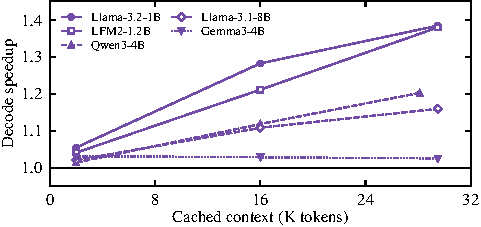
\includegraphics{fig/decode.pdf}
    \caption{Decode time per token against the length of the cached context, for the existing design and after our loop pass renames the keys, values, and scores into rings. Each point is the median of three runs of 250 tokens, and every step's logits are bit-identical between the two designs at every point. The annotation on each panel is the fitted cost per decoded position.}
    \label{fig:decode}
\end{figure}
% SOURCE: figs/data/decode-1b.json and decode-qwen.json, byte copies of amd-npu a6bc94b6 gate-R/1b-2026-10-21/gate-1b.json and 455740b1 gate-R/qwen-2026-10-21/gate-qwen.json; the figure plots the census (baseline) and R (our pass) arms and drops the 32,517 reproduction point, which repeats 32,512.
% DECISION: the event model's decode prediction and the cap-bounded estimate are not plotted. Neither is in these two records, and adding a line the data file does not carry would make the figure unreproducible from figs/data.

% VALUE: whole turns, against the existing program on its faster split: the gain rises with the cached context; at the traces' most common step it is moderate, and larger against the existing program on its default split; decode carries most of the gain and the composed prefill adds only at the largest steps; decode runs the hand renaming the pass matches; the handoff both sides pay, quoted so a reader can deflate the ratios
\label{subsec:turns}
The gain on a whole turn rises with the cached context.
Against the existing program on its faster split, OPCORD shortens a turn by $1.06$--$1.23\times$ at a 4{,}096-token context and $1.15$--$1.32\times$ at 16{,}384 on both LLMs, and by $1.33$--$1.34\times$ at 28{,}672 on the 1B, the one LLM we measure there (Figure~\ref{fig:turns}).
At the traces' most common step, about a thousand new tokens onto 16{,}384, a turn is $1.15$--$1.26\times$ shorter.
Decode carries most of the gain, since on renamed decode the composed prefill adds $1.09$--$1.10\times$ to steps of 4{,}096 tokens and nothing measurable to steps of up to 1{,}024.
In these turns, decode runs the renaming applied by hand, which our loop pass matches within 1\%.
% SOURCE: the composer over renamed decode on the existing S4 prefill: 1.088-1.098x at N = 4k, 0.993-1.004x at N <= 1k on both models (vault lab-agent-step (8), (10); amd-npu c61445d, 171082f).
% SOURCE: re-derived from the committed per-rep files (amd-npu c61445da turn-w3-1b.json, 171082f6 turn-w3-qwen.json), turn = median(append) + median(decode), best-vs-best = min over the two existing splits / min over the two composed ones, no handoff: Llama-3.2-1B 4k+512 1.096, 4k+1k 1.113, 4k+4k 1.229, 16k+512 1.256, 16k+1k 1.255, 16k+4k 1.316, 28k+512 1.336, 28k+1k 1.326; Qwen3-4B 4k+512 1.060, 4k+1k 1.076, 4k+4k 1.183, 16k+512 1.146, 16k+1k 1.150, 16k+4k 1.218. Against the existing default (its S2 with the unrenamed decode): 1B 1.118 / 1.157 / 1.460 / 1.374 / 1.500 / 2.173 / 1.435 / 1.513; Qwen 1.084 / 1.128 / 1.519 / 1.216 / 1.284 / 1.663; at 16,384 + 1,024 1.500 and 1.284.
% SOURCE: the turn harness runs census vs (c) decode (vault lab-agent-step (8), (10)); the loop pass's per-token time within 0.992-1.004 of (c) on the 1B and Qwen3-4B (lab-decode-long-context (22)).
% SOURCE: the 1B WITH its steady handoff, best-vs-best 1.088 / 1.104 / 1.215 / 1.235 / 1.236 / 1.295 / 1.307 / 1.300; handoff in the clean state 6.2-8.6% of the turn on the 1B and 3.4-8.2% on Qwen3-4B's clean cells (computed from the same per-rep files; the composed arm's smallest handoff per cell against its own turn).
% DECISION: 28,672 is quoted on Llama-3.2-1B alone, since Qwen3-4B has no cell there; the sentence says "the one LLM we measure there" rather than implying both.
% DECISION: the 1B's 16,384 + 4,096 existing-S2 run ran in the existing program's usual long-context mode (append 12.8-13.1 s), which D23 classes as representative rather than anomalous; its best-vs-best ratio takes the S4 arm and is unaffected. Qwen3-4B's 16k with-handoff ratios are not quoted (the handoff's page-fault state, Appendix handoff).

\begin{figure}[t]
    \centering
    % VALUE: the turn speedup over the step size and the cached context, placed on the traces' step distribution
    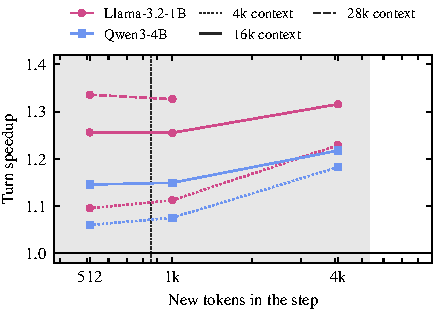
\includegraphics{fig/turns.pdf}
    \caption{Whole-turn speedup against the existing program on the faster of its two-column and four-column splits, by the number of new tokens in the step and the length of the cached context. A turn is its append and 250 decoded tokens, without the handoff of the KV cache. The shaded band spans the 25th to the 90th percentile of the new tokens per step in coding-agent traces and the dotted line is their median~\citep{zhu2026tracelab}.}
    \label{fig:turns}
\end{figure}

\subsection{Sources of the Gains}
\label{subsec:ablation}

% VALUE: what each part contributes: every prefill gain over the alternated baseline is the composer's reorder across column groups, which nothing hand-written or shipped does; the stream pass reproduces the alternation the baseline carries, so its gain over it is zero by construction, and the loop pass's decode renaming is the hand edit experts make, reaching FastFlowLM's time per token at long contexts; the passes' value is reach (§7.5, judged, not gains); the event model contributes the choices (§7.4)
Every prefill gain over the alternated baseline comes from the composer's reorder across column groups, which no hand-written or shipped design performs.
The two passes automate inside the compiler what experts do by hand, so their value is reach, applying an expert's edit legally to designs nobody tuned (Section~\ref{subsec:fidelity}).
The stream pass reproduces the hand alternation that the alternated baseline already carries, and the loop pass's renaming matches FastFlowLM's hand-tuned decode (Section~\ref{subsec:e2e}).
The event model contributes the choices, namely the split per regime and whether a removal pays (Section~\ref{subsec:accuracy}).

% VALUE: what contributes nothing to the prefill gain: packing alone, and the split (credited to neither side)
None of the gain comes from packing alone (Section~\ref{subsec:semantics}), and we credit the split to neither side, because the existing program's faster split flips with the regime as ours does (Appendix~\ref{app:split-first}).
% SOURCE: 16k + 4k append, composed on S4 vs composed on S2: Llama-3.2-1B 5,493.0 -> 2,950.8 ms (1.86x), Qwen3-4B 19,332.6 -> 10,342.7 ms (1.87x) (vault lab-split-sweep (4)-(5)); this is the split's own gain, credited to the regime and not quoted here.
% SOURCE: the shipped + Ar faster split equals the composer's faster split in 8 of 8 W1 cells (vault lab-split-sweep (18)) and 11 of 12 Table append cells (amd-npu 78ec55b7 E1 calls, the twelfth a near tie); Llama-3.1-8B 4k + 4k is the one other disagreement (Appendix split-first). Corrected 2026-10-22 (D19 convergence point 4).
% SOURCE: R-ship (the composed schedule at the existing program's per-chunk naming) equals the composer with rings within 0.1% (0.99996-1.00074, amd-npu 71081d1).
% DECISION: the split is a finding priced by the event model, not a removal over a baseline at its own faster split (D19 point 4); the reorder's gain is always quoted with each side at its own faster split.

% VALUE: the prefill reorder has two parts that the splits separate: within attention's two columns (the alternation the stream pass emits, measured against the existing program) and across column groups (the composer); at four columns the existing stream already alternates, so only the cross-group part remains; the within-operator share grows with the context while the cross-group share shrinks as attention takes over
In prefill, the reorder has one part between attention's two columns and one across column groups (Figure~\ref{fig:schedules}).
At the four-column split, the existing attention stream already issues two segments per column before it waits, so the hand alternation changes nothing there (Appendix~\ref{app:percell}).
The reorder across groups alone then gains $1.11$--$1.22\times$ from scratch and $1.33$--$1.46\times$ on appends on Llama-3.2-1B and Qwen3-4B, and on Gemma3-4B, whose attention stream has no wait to alternate at any split, it carries the whole gain.
At the two-column split, the alternation that the stream pass emits gains $1.12$--$1.42\times$ over the existing program and leaves $1.13$--$1.46\times$ to the reorder across groups.
The two parts move in opposite directions with the context, and on the append to 16{,}384 tokens the alternation gives $1.42\times$ and the reorder across groups $1.13\times$, since attention then holds most of the time.
% SOURCE: vault lab-split-sweep (22), medians of 5, the four cells being scratch 2,048 / scratch 4,096 / 4,096 + 4,096 / 16,384 + 4,096. At S4 shipped + Ar equals shipped within 0.0%, so composer over shipped is the cross-group reorder alone: 1B 1.13 / 1.22 / 1.46 / 1.33, Qwen 1.11 / 1.19 / 1.46 / 1.33. At S2 the order's gain splits into within-operator (shipped -> shipped + Ar) 1B 1.12 / 1.19 / 1.34 / 1.42, Qwen 1.13 / 1.20 / 1.37 / 1.42, and across-operator (shipped + Ar -> composer) 1B 1.25 / 1.45 / 1.37 / 1.13, Qwen 1.27 / 1.46 / 1.36 / 1.13.
% SOURCE: the segment counts are read from the existing attention streams at each split by our own analysis, and the equality is measured: at S4 shipped + Ar equals shipped within 0.1% on every cell of every model (vault lab-split-sweep (22)).
% DECISION: the 1.33x at 16,384 + 4,096 here is prefill TTFT and must not be conflated with a whole-turn ratio at a 28,672-token context.
% DECISION: the alternation is what the stream pass emits byte-identically on all 42 attention streams (Section 6); the text credits it as the within-operator removal, never as something the pass discovers.

\begin{figure}[t]
    \centering
    % VALUE: the decomposition in one picture: the composed schedule is below both existing schedules at every split of every
    % LLM, the hand alternation closes part of that distance only where attention has a wait to remove, and
    % which split is fastest is a property of the LLM rather than of the regime.
    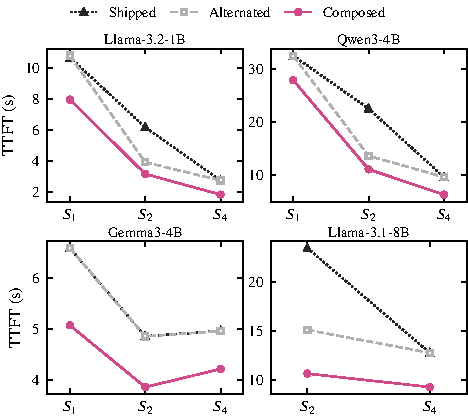
\includegraphics{fig/schedules.pdf}
    \caption{Time to the first new token by split, for the existing schedule, the existing schedule with attention's columns alternated by hand, and the composed schedule, on an append of 4{,}096 tokens to an 8{,}192-token context. $S_k$ gives attention $k$ of the eight columns. The existing and alternated schedules coincide wherever attention has no wait to alternate away, which is every split on Gemma3-4B and the four-column split on the others. Llama-3.1-8B is built on two splits only.}
    \label{fig:schedules}
\end{figure}
% SOURCE: figs/data/accuracy.json, the claimed and reported arms at cell append:8192:4096; the packed-into-one-command arm is not plotted because the only whole-model measurement of it predates the composer this paper evaluates, and Section~\ref{subsec:semantics} establishes at operator-pair scale that packing alone creates no overlap.


% VALUE: decode's gain needs the whole cycle renamed: keys and values alone gain nothing while the score buffer closes the cycle
In decode, renaming the keys and values alone, as a production mapping of another LLM does by hand~\citep{du2026gemma3}, is worth 0.3\%, because the shared score buffer still closes the loop's critical cycle, as the condition of Section~\ref{subsec:removal} requires.
% SOURCE: keys and values renamed with the existing score buffer kept: 1.002x (16,384) and 1.003x (32,512), tokens and logits bit-identical (vault lab-decode-long-context (28); amd-npu d8f0bd4c, score 5e1017a5); all three renamed (the loop pass): 1.269x / 1.391x (lab-decode-long-context (22)).

% VALUE: where removal does not pay, each with its measured reason: short appends where the composed pipeline is mostly fill and drain (the event model prices it right, and the turn still gains), and Llama-3.1-8B where both phases already read near the DRAM cap so only serialized compute remains to hide
Removal does not pay where a measured term leaves it nothing to hide.
At 512-token appends, the composed prefill runs at $0.88$--$0.93\times$ the existing order's speed, because with four chunks per layer its pipeline of in-flight commands is mostly fill and drain, which the event model prices correctly at all three contexts.
Llama-3.1-8B gains least from scratch, because its composed prefill already reads 93--96\% of the read cap.
% SOURCE: the 512-token appends, existing S4 faster at 0.88-0.93x (vault lab-agent-step (8), (10)); computed after the turns were measured, with the model unchanged (amd-npu e30be08 adds cell selection only; two earlier cells reproduce bit-identically): the model prices the existing S4 order below the composed one, 249.9 / 469.7 / 689.4 vs 294.7 / 513.6 / 732.4 ms at 4k / 16k / 28k (measured 265.0 / 482.1 / 699.7 vs 300.6 / 521.3 / 754.3), and the faster S4 order on 14/14 turn cells; at 1k appends its margin is 0.2-0.3%, inside its error, and choosing by it costs at most 23 ms of a turn (vault lab-agent-step (11), amd-npu 9d4f63f). Fill and drain: lab-agent-step (11), Section~\ref{subsec:removal}. Turn at 512-token appends, best-vs-best 1B 1.096 / 1.256 / 1.336, Qwen3-4B 1.060 / 1.146.
% SOURCE: 8B composer read rate over TTFT including host time, 51.5 GB/s at scratch 4,096 (its GEMM group 48.2) and 50.8 at scratch 2,048, against the 53.9-55.3 GB/s cap; bytes from the TXN BD chains over the measured TTFT (amd-npu 71901c50; vault lab-metric-fields (1), amendment 1).
% SOURCE: amd-npu 25f6adde decode-rename/w2c-8b-run-2026-10-22/score.json (vault lab-decode-long-context (44)). 16,384: baseline 192.617 ms/token, renamed 178.660, r median 1.0785 [1.0738, 1.0839], no-chain ceiling 1.0855. 30,720: 204.572 and 179.359, r 1.1397 [1.1356, 1.1511], ceiling 1.1597. Tokens and every step's logits identical across arms and repetitions. The partial arm on the same baseline and cells is 0.990x (lab-decode-long-context (19)).
% DECISION: the 512-token result is stated as a pricing checked against the measurement, not as a choice the system made during the runs.
% DECISION: the 8B decode is quoted as the bound predicting a small gain, never as a disappointment; the hand edit is the arm measured on that LLM, and the loop pass's 8B build is bit-identical but untimed.

\subsection{Model Accuracy and the Bound}
\label{subsec:accuracy}

% VALUE: the event model names the faster split in every case and orders every clearly separated pair; it prices the composed schedule within a few percent, always slightly high, and the baselines slightly low, so it understates gains; its value over interpolation is coverage: it prices, without running it, any configuration within each operator's probed range
The event model names the faster split in all 36 cases, one per append configuration of Table~\ref{tab:append} and schedule, against 27 for the better rule that always answers with one split, and orders all 83 pairs of schedules whose times differ by at least 5\%.
It prices the composed schedule at its chosen split within a median 2.15\% and a maximum 7.31\%, always slightly high, and the baselines a median 2.2\% low.
% SOURCE: scorer cp_score.py 86ba24b6 unchanged, output amd-npu 78ec55b7 prefill-overlap/cp-predict/score-2026-10-21.json, holds fd6e6c7b committed before reading; re-derived from that file: E1 36/36, constant-rule patterns 27 and 25, 33/33 excluding near-ties; E2 83/83 at a 5% gap; E3 (the composer at the model's chosen split) median 2.146%, max 7.311% (Qwen3-4B 8k + 4k), every one an over-prediction (+0.04% to +7.3%); baseline arms under-predicted, median -2.2% shipped and -2.1% shipped + Ar over 33 each; interpolation 2.30% against 1.95% on its 10 cells; E4 measured - predicted = +0.085 / +0.118 / +0.057 / +0.018 / +0.090 / +0.037 / +0.048 / +0.042 / +0.030 / +0.006 / -0.001 / +0.053 (vault lab-split-sweep (27)).

% VALUE: pricing each configuration beats a regime rule because the faster split varies with the LLM, not only with the regime; the event model's error grows only on schedules it never chooses; on a fifth LLM whose layers are not all attention it still names the faster split and orders the pairs
Pricing each configuration matters because the faster split varies with the LLM as well as with the regime.
On these appends Llama-3.2-1B and Qwen3-4B want four attention columns in every configuration and Llama-3.1-8B in seven of nine, whereas Gemma3-4B wants two in seven of nine.
Its error grows only on schedules it never chooses, such as those on the one-column split.
On LFM2-1.2B, whose layers are not all attention, it names the faster split in 7 of 8 cases, where the one exception is a pair 0.1\% apart, and orders all 19 pairs that differ by more than 5\%, at a median error of 2.6\%.
% SOURCE: computed from the same scorer output: measured faster split over the 36 calls is S4 in 27 and S2 in 9; by model, 9/9 S4 on Llama-3.2-1B and on Qwen3-4B, 7 of 9 S2 on Gemma3-4B, 2 of 9 S2 on Llama-3.1-8B; constant rules score S4 27, S2 9, S1 0.
% SOURCE: other arms (lab-split-sweep (27)): S1 under-predicted to -38.5% (1B 12k + 2k, shipped and shipped + Ar), the composer on S1 to -31.8%; shipped on S2 -15.2% (8B 8k + 4k), -20.4% (1B 12k + 2k), -14.6% (Qwen3-4B 8k + 4k); none is ever the best split. The existing order's alternation ratio is lower at the 1B's mid-range chunks (0.41-0.57 against 0.66-0.68; lab-agent-step (4)), which the probes of a 2,048-token prompt do not see; no cause is claimed in the text.
% SOURCE: LFM2-1.2B, amd-npu e695d3dd rerun-2026-10-22/g1-score.json (output 838a2220 committed before reading; predictions g1-predictions.json sha256 377c31ff... reproduced byte-for-byte by the scorer): winner 7 of 8, the single miss at scratch 2k shipped (S1 predicted, S2 measured, gap 0.09%); signs 19 of 19 at a 5% threshold; 24 cell errors, median 2.6%, max 37.2% (16k + 4k shipped on the one-column split).
% DECISION: this answers the comparator objection with the grid's own data rather than by asserting the model is better; the regime rule is the paper's own explanation, so it is scored, not waved aside.
% DECISION: LFM2 is reported for prefill only; no turn has run for it and none is claimed. Its large errors are stated rather than excluded, since they fall on arms the composer never chooses and the direction is under-prediction.

\begin{figure}[t]
    \centering
    % VALUE: predicted against measured TTFT on every schedule of the append configurations; the points off the band are schedules the event model never chooses
    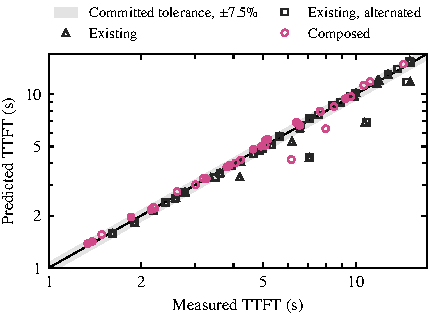
\includegraphics{fig/accuracy.pdf}
    \caption{Predicted against measured TTFT on appends across four LLMs, three schedules, and three splits, with a band of $\pm7.5\%$. The points well below the band are schedules on the one-column attention split, which the event model never chooses, and the existing program on the two-column split at 8{,}192- and 12{,}288-token contexts, which it prices 15--20\% low.}
    \label{fig:accuracy}
\end{figure}

% VALUE: once the order is right a column group, not the CP, binds the lower bound, and which group binds flips with the workload, which is what moves the faster split; the composed schedule lies within a modest factor of the bound, which the event model places closely and never below; no run beats its bound; read as a gap, most of the distance is closed on the dense LLMs and the rest is the overlap's price and unhidden CP and host work
\label{subsec:bound-eval}
Once the order is right, a column group's busy time rather than the CP binds the lower bound, and which group binds flips with the workload.
On Llama-3.2-1B and Qwen3-4B, the GEMMs bind from scratch at 2{,}048 tokens and attention on an append to 16{,}384, at every split, which is why the faster split moves from two attention columns to four (Section~\ref{subsec:split}).
On the twelve appends of Table~\ref{tab:append}, the composed schedule lies $1.17$--$1.63\times$ above the bound, and none of the 33 runs that test the bound ran faster than it (Appendix~\ref{subsec:tests}).
Read as a gap, the schedule closes a median 65\% of the distance from the alternated baseline to the bound, and 34--76\% across these appends, most on the dense LLMs and least on Gemma3-4B, whose windowed attention leaves the GEMMs binding.
What remains is the price of overlap under the DRAM read cap, 1.0--5.1\% of TTFT where the GEMMs bind, and the CP's and the host's work that the schedule does not hide.
% SOURCE: computed in aie-cosched-paper-0 tmp/regime/cells.py over the 24 committed bound cells (2 models x 3 splits x 4 configurations, vault lab-split-sweep (8) / ch3-formulation G6): the binding term is the GEMMs in 12 cells and attention in 12; 1B at 2,048 from scratch the GEMM term rises 377 / 413 / 564 ms from S1 to S4, and on a 16,384 + 4,096 append attention falls 10,776 / 5,258 / 2,631 ms.
% SOURCE: re-derived from amd-npu 78ec55b7 score-2026-10-21.json and checked against Table append (composed / bound = 1.166-1.631; the earlier SOURCE here read 1.196, which is the 1B 2k + 4k cell, not the minimum): predicted minus measured over all 12 is +0.000 to +0.088, median 0.025, never negative; B1 0 violations over 33 runs, the lowest ratio 1.023 (vault lab-split-sweep (27)).
% SOURCE: gap captured, per cell: baseline = the faster of the shipped arms over the three splits, ours = the faster composed arm, floor = the smallest lower bound over the three splits, captured = (baseline - ours) / (baseline - floor). Llama-3.2-1B 70 / 72 / 43%, Qwen3-4B 71 / 75 / 46%, Gemma3-4B 55 / 44 / 34%, Llama-3.1-8B 76 / 73 / 61% at 2k+4k / 8k+4k / 12k+2k; median 65%; the dense LLMs 70-76% on six of their nine cells.
% SOURCE: applying 0.085 x the co-runner where the GEMMs bind gives 6.4-269.2 ms, 1.0-5.1% of TTFT, tightening the gap to the bound from a median 1.23 to 1.17 on those cells; the unhidden CP and host residual is 63-264 ms on the 1B's non-anomalous cells and 139-741 ms on Qwen3-4B's (tmp/regime/cells.py, as above).
% COMMENT: two of the 24 cells are already-excluded artifacts, not evidence: the 1B's S1 16,384 + 4,096 cell ran in the intermittent slow state the record does not quote, and Qwen3-4B's S1 16,384 + 4,096 measures 0.98 of its own bound, which lab-split-sweep (8) records as the bound not being strict where attention is extrapolated tenfold.
% DECISION: the ratio to the bound is the bound at the composed schedule's own split, as Table append reports it; the gap fraction uses the smallest bound over the splits and the stronger baseline, the conservative reading of both.

% VALUE: three hand-written designs put each class of the two cells that hold no costly instance on the critical path and test the textbook condition directly: a removal off the binding cycle is worth nothing, the set that cuts it pays, and a class pays only where it binds
\label{subsec:synthetic}
Three small designs of our own put the two remaining cells of Table~\ref{tab:grid} on the critical path.
Where two name dependences close one cycle through a core, removing either alone gains nothing measurable, whereas removing both gains up to $1.60\times$.
An order dependence inside a loop gains $2.00\times$ where it closes the producer--consumer cycle, and nothing where each core's own loop binds instead.
Each outcome follows from whether the removal cuts the binding cycle (Appendix~\ref{app:synthetic}).
% SOURCE: re-derived from the committed scores (amd-npu 2ea67242 and c4f9a19d, runs-2026-10-22/{aon,ns,ol}/score.json; designs c423a98b, 9c94988a, ea3316e4; all three holds rc 0, no faults, every per-tile output check true). s1 by level, g(2,1) / g(1,2) / g(2,2): m256p1 1.0096 / 1.0031 / 1.5970; m1024p1 1.0003 / 0.9980 / 1.1458; m1024p4 0.9824 / 0.9876 / 1.0312. s2: single-indep 59.21, ring-indep 58.45 ms, g 1.0130, repetition spread 1.5-2.0%. s3: stream-s2 3.610, pair-s2 7.235, stream-s4 11.653, pair-s4 11.643 ms, g 2.0044 and 0.9991 (vault lab-synthetic-classes (4)-(6)). The 1.60x rests on a depth-one baseline whose repetitions span 193% of their median (Appendix synthetic).
% DECISION: no design, depth, or work level was changed after its own measurement, since a design altered after it ran stops being evidence for its class; the slow-side single removals at the third work level are stated with their sizes.

\subsection{Fidelity and Reach}
\label{subsec:fidelity}

% VALUE: the method reads exactly what each stack dispatches: 625 streams of three toolchains re-emit byte for byte, and nearly every wait in 792 streams is attributed to a mechanism, with the residual located; the three stream counts (625 round trip, 792 analysed, 277 in the census) related once, by scope
Because the method starts from streams a stack has already emitted, it must read them exactly, and it does so on all three toolchains.
Re-emitting 625 streams byte for byte shows that the analysis starts from exactly what each stack dispatches, namely 375 streams built by MLIR-AIR and 218 recorded from FastFlowLM, both through the lifter of Section~\ref{subsec:closed}, and 32 built by IRON through IRON's own translator.
Over 792 streams, the analysis attributes 73{,}994 of 74{,}010 waits to one of its ordering mechanisms.
% SOURCE: recording libhrx (FastFlowLM 44d01787, gemma4e-flash), every prompt length 1-1,024 recorded with 0 /dev/accel opens; 8 buckets, 218 distinct streams, round trip and identity 218 / 218 (vault lab-cosched-passes (14)); lifter fix mlir-aie 91f64387ffb, 375 / 375 MLIR-AIR streams byte-identical (lab-cosched-passes (3)); IRON 32 / 32 through its own translator (1-intro SOURCE). Further populations not counted here are in Appendix roundtrip.
% SOURCE: aie-cosched results/2026-10-23-s35-data, registered c57b708, result ef6733a (aie-cosched-stream-deps at mlir-aie 0489d325082): waits 74,010, attributed 73,994; unattributed waits 16 (4 in each of the 4 MLIR-AIR fused-decode streams) and unattributed ops 67 (66 there, 1 IRON); per population AIR 10,256 / 10,240, FLM 63,392 / 63,392, IRON 362 / 362; one IRON stream (179,576 ops) not analysed; 792 streams read.
% SOURCE: 792 = 543 MLIR-AIR + 218 FastFlowLM + 31 IRON analysed streams (aie-cosched 93f491b, mlir-aie f9ad95dc02f, lab-cosched-passes (62), P7c; 4-method Textbook Classes SOURCE); 277 = 27 MLIR-AIR + 32 IRON + 218 FastFlowLM (lab-cosched-passes (41)); 625 = 375 + 218 + 32 (lab-cosched-passes (3), (9), (14)).
% DECISION: the attribution counters are the analysis's edge-level coverage; they are a different quantity from the census's instance count, and the two must not be conflated in the text.

% VALUE: the census: at stream granularity our stream pass, run over 277 streams of three stacks with the known instances excluded, removes no further instance; the zero describes the pass's lane rule (a lane defined), not the streams; the residual bookkeeping is in the appendix
\label{subsec:census}
Beyond the instances of Table~\ref{tab:grid}, the stream pass proposes moves on 29 of 277 streams of the three stacks, and its checker and an independent second implementation (Section~\ref{subsec:checkers}) agree on every verdict, refusing FastFlowLM's 16, which would overflow a channel's task queue, and accepting IRON's 13.
% SOURCE: population 277 = 27 MLIR-AIR + 32 IRON + 218 FastFlowLM (vault lab-cosched-passes (41) and its addendum). aie-cosched tools/oracle_results/2026-10-21-d3 prex_scan.json: monotone proposals 0 on all 277; full-mode moves on 29 (16 FastFlowLM wait-free-lane hoists, 13 IRON in-block moves) (foundation audit 2026-10-22, Phase 2.B J7).
% SOURCE: aie-cosched 9912aa9 (lab-cosched-passes (62), the iron13 run): the 13 IRON moves ACCEPTED by the C++ checker and legality.check on each stream's own configuration (3 binary_elementwise on their xclbin and routed device; 10 decode-fused_op on the device whose runtime sequence has the stream's skeleton), none crossing a wait; worth unpriced.
% SOURCE: aie-cosched baf37e0 (lab-cosched-passes (62), P7b): lanes.json byte-equal to the reviewer's 8da59d9a (247 / 29 / 1 streams with 1 / 2 / 0 lanes); the 16 two-lane production-engine streams REFUSED on all 16 by legality.check (full, configured) and the C++ checker with identical decided codes: QUEUE-OVERFLOW on the 8 of columns 0/3, QUEUE-OVERFLOW + FENCE-CROSSED-UNPROVEN on the 8 of columns 6/7, no BD-REUSE.
% SOURCE: the lane rule is (35). Breakdown: 199 single-lane by the lane rule (193 production + 6 IRON gemm + 1 other), 61 single-phase (60 issuing nothing after the first wait, plus IRON decode-fused_op fc078b33, 179,576 ops, unplaced), 16 with queue overflow. The characterization is B-prime (vault (46)): 193 of 218 with at least one accepted reordering at 1.000-1.0069, IRON 0 of 84 accepted (all queue-overflow), MLIR-AIR none proposed.
% DECISION: the census reports the pass's proposals and verdicts, not a census zero; at loop granularity the text states what the analysis judges.
% DECISION: the census() procedure as first specified is NOT-READY on the committed artifacts (its pre-scan commit was never made); the text reports the pass's offline steps, which ran with the same pass and checkers, and never calls the zero the result of that procedure.

% VALUE: at loop granularity the analysis judges every loop of the MLIR-AIR designs and part of IRON's, with the reason for the rest; our passes judge MLIR-AIR designs of LLMs never examined, with no gain claimed; the reach differs by what each toolchain exposes
At loop granularity, the analysis judges all 3{,}719 loops of the MLIR-AIR prefill and decode designs, and 50 of IRON's 242, whose others hold a lock across an inner loop with a trip count the dispatch does not give.
Our passes also judge the MLIR-AIR designs of five LLMs we never ran or examined, Llama-3.2-3B, Phi-4-mini, Qwen2.5-3B and~7B, and Qwen3-8B.
On their decodes the loop pass renames attention's keys, values, and scores as on the evaluated LLMs and finds every other loop's buffers already multi-slot, and on three of their prefills it judges every loop, but we claim no gain on any of them.
The method's reach thus follows what each toolchain exposes, since we read and rewrite MLIR-AIR's designs, read and check IRON's, and read and classify FastFlowLM's (Section~\ref{subsec:closed}).
% SOURCE: aie-cosched results/2026-10-23-s35-data, registered c57b708, result 3dbc1ee (mlir-aie dev 027651259b5): MLIR-AIR prefill 3,488 / 3,488 judged over 109 designs (1,184 single-slot renamable), the nine fused decodes 231 / 231 (102), IRON 50 / 242 (192 refused: an inner lock-holding loop whose trip count is not derivable from the dispatch).
% SOURCE: P8 (a), the unexamined MLIR-AIR models (aie-cosched e5ad472; expectations committed before the runs; 0 accel opens; kernels byte-identical): 5 decodes (Llama-3.2-3B, Phi-4-mini, Qwen2.5-7B / 3B, Qwen3-8B), the attention ring renamed, 12 buffers (6 on Qwen2.5-3B); 3 prefills (Llama-3.2-3B, Phi-4-mini, Qwen3-8B), every loop judged, single-slot renamable buffers only the GEMM output tiles, 168 / 168 / 144, worth unpriced. Ruling 3 (registered 7687182, results/2026-10-23-phase-rerun; mlir-aie 0c5e8e37fac / 6b9e6666991, lit 46/46): on all nine fused decodes every loop is judged, 0 refused, and the projection loops' name buffers are all multi-slot already (vault decisions log, P8 (a) and Ruling 3).
% SOURCE: FastFlowLM's closed libraries build its streams and buffers, so removals are measured on MLIR-AIR's fused prefill, which reimplements FastFlowLM's designs (mlir-air llms README; Section~\ref{subsec:closed}).
% DECISION: the designs never examined are judged by the passes, never credited with a gain (contract, "No overclaim"); no device run exists for them.

\subsection{Overheads}
\label{subsec:overheads}

% VALUE: OPCORD's own costs are one-time per prompt shape or per LLM and split, outside the measured call except a small binding step that every TTFT includes; even charged per request the composed schedule stays ahead of the existing program on the two-column split (a different baseline, named); memory and switching costs are priced in the appendix
OPCORD's costs are paid once per prompt shape, LLM, and split, and they stay below its gains even when charged on every request.
On the two-column split, composing a shape's commands takes 56--148\,ms on Llama-3.2-1B and 143--368\,ms on Qwen3-4B, and planning it 63--206\,ms and 0.3--1.1\,s; later prompts of that shape reuse this work, whereas an agent's turn, whose cached context grows, pays it each time.
Charged on every request, the composed schedule still leads the existing program on that split by $1.13$--$2.18\times$ at every configuration we measure.
Every TTFT includes the 7--50\,ms that binding attention's positions takes inside the call.
Probing each operator alone costs 9--39\,s, paid once per LLM and split.
Appendices~\ref{app:rings} and~\ref{app:relayout} price the memory and the switches between splits.
% SOURCE: composition measured host-only before and after the operator-level cache (amd-npu 82c5b5b0, compose-gate-2026-10-22/; stand-in pyxrt). Gate: 56 cells over 5 models and 14 builds, 65,550 commands and 325,974,776 words, every command byte-identical to the previous path, so every device measurement we hold is unaffected. S2 composition: 1B 56 / 148 / 140 / 128 ms; Qwen 143 / 368 / 240 / 297 ms at scratch 2k / scratch 4k / 4k+4k / 16k+4k. Per-request bound against the run medians and the shipped arm's own first-call extra: 1B 1.18 / 1.31 / 1.64 / 2.18, Qwen 1.13 / 1.26 / 1.53 / 1.51. The shipped arm's own per-call composition, from its first call against its later ones, is -80 to +87 ms (Appendix overheads).
% SOURCE: planning 63-206 ms (1B) and 0.3-1.1 s (Qwen3-4B); bind step 7-14 ms (1B) and 15-50 ms (larger models); probes 9-39 s per model and split (vault lab-split-sweep (29)-(30)).
% DECISION: planning is the larger one-time term and is left as it is; it makes no cell a loss, and the paper does not claim the prototype is fast, only that its cost is one-time and bounded.
% DECISION: Table 2 (overheads) stays dropped. Four of its five rows restate numbers stated beside the design decision they price, and the fifth, planning time, is answered here.
% COMMENT: the planning VERIFY that stood here is answered for the two-column split (lab-split-sweep (29)-(30)). Open (foundation audit 2026-10-22, B37): the per-request charge is not computed on the four-column split the composer takes for appends, where composition alone is 131-214 ms (1B) and 236-567 ms (Qwen3-4B).

% MERGED 2026-10-22 into 2-background.tex as a subsection, per MLSys convention. Nothing was cut.

\section{Conclusion}
\label{sec:conclusion}

% VALUE: one paragraph: concurrency on a spatial array is free in the hardware but rationed by false dependences, at one in-order CP and inside operators' loops; reordering issue, renaming buffers, and choosing the split per regime recover what the expert designs leave idle, bit-identically, from probes alone; what remains (host work between commands, decode's weight reads); no outlook, which the discussion carries
% DECISION: written with the evaluation.
\E{Conclusion: written with the evaluation.}


\bibliography{refs}
\bibliographystyle{mlsys2025}

% VALUE: the venue requires a section after the references describing how generative AI was used, covering code,
% data, writing, ideation, literature search and experiment design. Modelled on the author's FPGA'27 paragraph
% ("We use AI coding agents to write our passes, the measurement harness, and the scripts..."), extended to the
% activities this call names, and framed as assistance: the authors set the direction and own every decision.
% DECISION: author to review and amend before submission; this is the authors' own statement, not a drafted claim.
\section*{AI Usage Disclosure}

We used AI coding agents as tools, under the authors' direction and within a protocol the authors set.
The agents wrote the compiler passes, the measurement harness, and the scripts that analyse measurements, implement the event model, and draw the figures.
They ran the experiments on hardware the authors released to them for each run, checked each run against gates the authors specified, and maintained the records those gates produce.
They also searched for related work, proposed candidate experiments and designs, and drafted and revised the text of this paper.

The research direction, the claims, and the scope of what is measured and reported are the authors' own.
The authors decided which experiments to run and which to stop, which results to quote and which to withhold, and how every claim is qualified.
Each number in this paper was re-derived from the committed measurement artefacts rather than accepted from an agent's summary, and the predictions registered before the runs, the exclusions, and the limitations stated throughout the paper are the authors' decisions.


\end{document}
